\chapter{“1+1”维波动问题完全弱形式时空混合有限元法}
本章为进一步分析弹性波动力问题在复杂区域求解，
引入时间方向的网格与空间方向的网格构成“1+1”形式的二维网格来离散计算。
对网格的节点个数、布置方式、网格形状等元素进行调控来模拟各式各样的复杂求解域。
并在这套网格的基础上，采用基于哈密顿原理的完全弱形式伽辽金法进行求解。
FIXME: 施加虚位移边界条件。
对上一章解决时间末端边界问题的拉格朗日乘子法进行测试并分析，
为这套解决方案提供更为坚实的理论基础和实际依据。

\section{一维波动问题及时间强形式求解方案}

不失一般性，考虑如图\ref{fg:yiweibodongwenti}所示的一维弹性杆问题，
该弹性杆的材料密度为$\rho$、弹性模量为$E$、横截面积为$A$，杆受沿$x$方向的体力$b$和在$x_t$处的外面力$P$作用。
左端为固定端$x_g$，右端为自然边界$x_t$。

\begin{figure}[!h] 
    \centering
    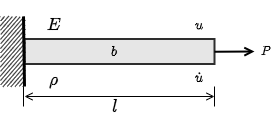
\includegraphics[scale=0.9]{fig/一维波动问题示意图.png}
\caption{\centering{一维弹性杆问题示意图}}
\label{fg:yiweibodongwenti}
\end{figure}

在式\eqref{eq:functional}的哈密顿原理中，
弹性杆系统中的哈密顿量$\Phi$以及内部的动能$T$和势能$U$的分别为:
\begin{equation}\label{eq:phi}
    \Phi = \int_{t_0}^{t_1} T - U dt
\end{equation}
\begin{equation}\label{T_2d}
    T = \int_{x_0}^{x_1} \frac{1}{2} \rho A \dot u^2 dx
\end{equation}

\begin{equation}\label{U_2d}
    U = \int_{x_0}^{x_1} \frac{1}{2} EA u_{,x}^2 dx
    -\int_{x_0}^{x_1} ub dx  + uP \vert_{x=x_t}
\end{equation}
式中，$u$和$\dot u$为位移及其速度，
$u_{,x}$为位移对$x$的一阶导数，即应变。

根据哈密顿原理，引入变分运算，可以得到相对应的泛函问题：
找到一个$u \in \mathcal U$使得，
\begin{equation}\label{eq:1d weak form}
    \begin{aligned}
        \delta \Phi (u) &= \int_{t_0}^{t_1} \int_{x_0}^{x_1} (\delta \dot u \rho A \dot u - \delta u_{,x} EA u_{,x}) dx dt \\
        &- \int_{t_0}^{t_1} (\int_{x_0}^{x_1} \delta ub dx  + \delta uP \vert_{x=x_t})dt \\
        &= a(\delta u, u) - f(\delta u) \\
        &=0
    \end{aligned}
    \quad
    \forall \delta u \in \mathcal V
\end{equation}

为进一步验证其与欧拉-拉格朗日方程之间的等价性，对弱形式\eqref{eq:1d weak form}进行分部积分，可得：
\begin{equation}
    \begin{aligned}
        & - \int_{t_0}^{t_1} \int_{x_0}^{x_1} \delta u (\rho A \ddot u - EA u_{,xx} - b) dx dt \\
        & + \int_{x_0}^{x_1} \delta u \rho A \dot u n_t dx \vert_{t_0}^{t_1}
        - \int_{t_0}^{t_1} \delta u (EA u_{,x} n_x \vert_{x_0}^{x_1} - P) dt
        &= 0
    \end{aligned}
\end{equation}
其中，$n_t$和$n_x$分别为单位外法向量在时间和空间维度上的分量。
根据哈密顿原理虚位移在时间端点处为零：
\begin{equation}\label{eq:1d_virtual_BC}
    \delta u\vert_{t=t_0} = \delta u\vert_{t=t_1} = 0
\end{equation}
同时，由于$\delta u$在位移边界条件处$x=x_g$也必须为零，即$\delta u\vert_{x=x_0}=0$，因此可以得到：
\begin{equation}
    EA u_{,x} n_x \vert_{x=x_t} = P
\end{equation}
最终，哈密顿原理\eqref{eq:1d weak form}所应用的欧拉-拉格朗日方程强形式为：
FIXME
\begin{equation}
    \left \{
    \begin{aligned}
        &\rho A \ddot u = EA u_{,xx} + b, \quad & (x,t) \in \Omega \\
        &u\vert_{x=x_g} = u_g, \\
        &EA u_{,x} n_x \vert_{x_t} = P \\
        &u\vert_{t=t_0} = u_0, \\
        &\dot u\vert_{t=t_0} = \dot u_0
    \end{aligned}
    \right .
\end{equation}

在传统有限元法在求解上述问题时，通常采用时间域强形式离散与空间域弱形式离散相结合的方法，
即在时间维度采用分部积分而空间部分不变。
此时，式\eqref{eq:1d weak form}可改写为：
\begin{multline}
    \int_{t_0}^{t_1} \int_{x_0}^{x_1} \delta u \rho A \ddot u dx dt + \int_{t_0}^{t_1} \int_{x_0}^{x_1} \delta u_{,x} EA u_{,x} dx dt = \\ 
    \int_{x_0}^{x_1} \delta u \rho A \dot u n_t dx \vert_{t_0}^{t_1}
    + \int_{t_0}^{t_1} \delta u P\vert_{x=x_t} dt + \int_{t_0}^{t_1} \int_{x_0}^{x_1} \delta u b dx dt
\end{multline}
引入哈密顿原理的时间虚位移边界条件$\delta u(t_0) = \delta u(t_1) = 0$，得到如下弱形式：
\begin{multline}
    \int_{t_0}^{t_1} \int_{x_0}^{x_1} \delta u \rho A \ddot u dx dt + \int_{t_0}^{t_1} \int_{x_0}^{x_1} \delta u_{,x} EA u_{,x} dx dt = \\ 
    \int_{t_0}^{t_1} \delta u P\vert_{x_t} dt + \int_{t_0}^{t_1} \int_{x_0}^{x_1} \delta u b dx dt
\end{multline}
对上式采用配点法进行时间维度离散，要求在给定的任意$t = t_{n+1}$时刻满足：
\begin{equation}\label{eq:1d_iter_weak_form}
    \int_{x_0}^{x_1} \delta u \rho A \ddot u dx + \int_{x_0}^{x_1} \delta u_{,x} EA u_{,x} dx = 
    \delta u P\vert_{x_t} + \int_{x_0}^{x_1} \delta u b dx 
\end{equation}

进一步引入有限元离散近似位移$u$、速度$\dot u$及加速度$\ddot u$，有：
\begin{equation}\label{eq:uh1D}
    \left \{ 
        \begin{aligned}
        u^h(x,t_n) &= \sum_{I=1}^{n_p} N_I(x) u_{In} \\
        \dot u^h(x,t_n) &= \sum_{I=1}^{n_p} N_I(x) \dot u_{In} \\
        \ddot u^h(x,t_n) &= \sum_{I=1}^{n_p} N_I(x) \ddot u_{In}
        \end{aligned}
    \right .
\end{equation}
式中，$N_I$表示空间域内的有限元形函数；$n_p$表示节点总数；
$u_{In}$、$\dot{u}_{In}$和$\ddot{u}_{In}$分别表示在$t_n$时刻的位移、速度和加速度。

将式\eqref{eq:uh1D}代入\eqref{eq:1d_iter_weak_form}可得离散控制方程：
\begin{equation}\label{Mu+Ku=f}
\boldsymbol M \ddot{\boldsymbol u}_{n+1} + \boldsymbol K \boldsymbol u_{n+1} = \boldsymbol f_{n+1}
\end{equation}
其中，$\boldsymbol M$为质量矩阵，$\boldsymbol K$为刚度矩阵，$\boldsymbol f_{n+1}$为$t_{n+1}$时刻的力向量。
它们的分量表达式如下：
\begin{equation}
    \left \{ 
        \begin{aligned}
        M_{IJ}  &= \int_{x_0}^{x_1} \rho A N_I N_J dx \\
        K_{IJ}  &= \int_{x_0}^{x_1} EA N_{I,x} N_{J,x} dx \\
        f_{I}   &= \int_{x_0}^{x_1} b N_{I} dx + N_{I} P\vert_{x_t}  
        \end{aligned}
    \right .
\end{equation}
而$\boldsymbol u_{n+1}$和$\ddot {\boldsymbol u}_{n+1}$为$t_{n+1}$时刻的位移及其加速度：
\begin{equation}
    \left \{ 
        \begin{aligned}
        \boldsymbol u_n &= \{u_{1n}, u_{2n}, \cdots, u_{n_p n}\}^T \\ 
        \ddot {\boldsymbol u}_{n+1} &= \{\ddot u_{1n}, \ddot u_{2n}, \cdots, \ddot u_{n_p n}\}^T 
        \end{aligned}
    \right .
\end{equation}

采用Newmark-$\beta$法对式\eqref{eq:1d_iter_weak_form}进行求解时，位移、速度和加速度采用如下差分格式进行近似：

\begin{equation}\label{3.2}
\left \{
\begin{split}
\ddot{\boldsymbol{u}}_{n+1} &= \boldsymbol{M}^{-1}(\boldsymbol{f}_{n+1} - \boldsymbol{K} \boldsymbol{u}_{n+1})  \\
\dot{\boldsymbol{u}}_{n+1} &= \dot{\boldsymbol{u}}_n + \Delta t ((1 - \gamma)\ddot{\boldsymbol{u}}_n + \gamma\ddot{\boldsymbol{u}}_{n+1}) \\
\boldsymbol{u}_{n+1} &= \boldsymbol{u}_n + \Delta t \dot{\boldsymbol{u}}_n + \frac{\Delta t^2}{2} \left( (1 - 2\beta)\ddot{\boldsymbol{u}}_n + 2\beta\ddot{\boldsymbol{u}}_{n+1} \right)
\end{split}
\right .
\end{equation}
FIXME
其中，$\Delta t$为时间步长。
$\beta$和$\gamma$为Newmark参数，通过调整这两个参数，可切换显隐式求解。
其中，当$\gamma = \frac{1}{2}$、$\beta = 0$时为条件稳定的中心差分法。

联立空间离散方程式\eqref{Mu+Ku=f}与时间离散格式\eqref{3.2}，整理可得到一维弹性杆问题的Newmark-$\beta$法迭代公式：
\begin{equation}\label{3.5}
\left \{
\begin{split}
\left(\boldsymbol{M} + \frac{\gamma \Delta t}{\beta} \boldsymbol{K}\right)\ddot{\boldsymbol{u}}_{n+1} &= \boldsymbol{f}_{n+1} - \boldsymbol{K}\left(\boldsymbol{u}_n + \Delta t \dot{\boldsymbol{u}}_n + \frac{\Delta t^2}{2}(1 - 2\beta)\ddot{\boldsymbol{u}}_n\right) \\
\boldsymbol{u}_{n+1} &= \boldsymbol{u}_n + \Delta t \dot{\boldsymbol{u}}_n + \frac{\Delta t^2}{2}\left((1 - 2\beta)\ddot{\boldsymbol{u}}_n + 2\beta\ddot{\boldsymbol{u}}_{n+1}\right) \\
\dot{\boldsymbol{u}}_{n+1} &= \dot{\boldsymbol{u}}_n + \Delta t\left((1 - \gamma)\ddot{\boldsymbol{u}}_n + \gamma\ddot{\boldsymbol{u}}_{n+1}\right) \\
\end{split}
\right .
\end{equation}




\section{一维波动问题的拉格朗日乘子型时空混合离散分析方法}

\subsection{拉格朗日乘子型虚位移边界条件施加方案}

为了建立完全弱形式下的时空混合离散(时间维度和空间维度均不做分部积分)，
必须得施加虚位移边界条件\eqref{eq:1d_virtual_BC}。
本小节将第\ref{ch:1dimension}章所提基于拉格朗日乘子的时域末端本质边界条件施加方案，
引入到泛函变分方程\eqref{eq:1d weak form}中，
从而构造全新路径来施加虚位移本质边界条件。

首先，为了表述方便，这里引入双线性算子表示哈密顿量\eqref{eq:phi}。
需要注意的是，为满足全域的变分一致性，哈密顿量中需要补充初始动量自然边界条件，此时哈密顿量可表示为如下形式：
\begin{equation}\label{eq:hmd}
    \Phi(u) = \frac{1}{2} a(u,u) - f(u)
\end{equation}
其中，$a(\bullet,\bullet):\mathcal U \times \mathcal U \rightarrow \mathbb R$为双线性算子，$f(\bullet):\mathcal U \rightarrow \mathbb R$为线性算子，其表达式如下所示：
\begin{equation}
    a(u,u) = \int_{t_0}^{t_1} \int_{x_0}^{x_1} (\dot u \rho A \dot u - u_{,x} EA u_{,x}) dx dt
\end{equation}
\begin{equation}
    f(u) = 
    - \int_{x_0}^{x_1} u \rho A \dot u_0 \vert_{t=t_0} dx
    - \int_{t_0}^{t_1} \left (\int_{x_0}^{x_1} ub dx  + uP \vert_{x=x_t}\right )dt
\end{equation}

在有限元离散的完全弱形式\eqref{eq:1d weak form}试函数近似空间$\mathcal{U}_h$和权函数近似空间$\mathcal{V}_h$并不相同，权函数近似空间$\mathcal V_h$要求其任意元素在时间末端处为零，即$\delta u(x,t_1)=0$。
此时，将传统能量泛函\eqref{eq:1d weak form}中的虚位移$\delta u$作为拉格朗日乘子，并将其采用$v$表示。
进一步，将该拉格朗日乘子项引入式\eqref{eq:hmd}中的哈密顿量，可得如下全新能量泛函表达式：
\begin{equation}\label{3.16}
\bar \Phi(u,v) = \frac{1}{2}a(u,u) - a(u,v) + f(v)
\end{equation}
对上述双变量能量泛函进行变分，
并考虑$\delta u$和$\delta v$的任意性，引入相同的有限元离散近似$u$和$v$，即$u_h$和$v_h$，可得如下伽辽金弱形式：
找到一组解$u_h \in \mathcal{U}_h, v_h \in \mathcal{V}_h$，使得
\begin{equation}\label{3.21}
    \left \{
    \begin{aligned}
        a(\delta u_h, u_h) - a(\delta u_h, v_h) &= 0, \quad & \forall \delta u_h \in \mathcal{U}_h \\
        -a(u_h, \delta v_h) &= -f(\delta v_h), \quad & \forall \delta v_h \in \mathcal{V}_h
    \end{aligned}
    \right .
\end{equation}

在采用时空混合有限元法进行分析时，对位移变量$u$进行的有限元近似，
区别于之前的近似表达式\eqref{q_h}和\eqref{dotq_h}所示的单一维度近似，
此处的形函数$N_I(x,t)$为时空二维结构，其对应的近似值$u^h$的表达式如下：
\begin{equation}\label{uv_h}
u^h (x,t) = \sum_{I=1}^{n_p} N_I (x,t) d_I
\end{equation}
对时间的一阶导数的近似值$\dot u^h$为：
\begin{equation}\label{dotuv_h}
    \dot u^h = \sum_{I=1}^{n_p} N_{I,t} d_I
\end{equation}
对位移的一阶导数的近似值$u_{,x}^h$为：
\begin{equation}\label{uv_x^h}
    u_{,x}^h= \sum_{I=1}^{n_p} N_{I,x} d_I
\end{equation}
$N_{I,x}$为形函数对位移的导数。
通过有限元近似表达式，可得到对应的离散控制方程为：
\begin{equation}
\begin{bmatrix}
\boldsymbol K & -\boldsymbol K \\ -\boldsymbol K & \boldsymbol 0
\end{bmatrix}
\begin{Bmatrix}
\boldsymbol u \\ \boldsymbol v
\end{Bmatrix} =
\begin{Bmatrix}
 \boldsymbol 0 \\ -\boldsymbol f
\end{Bmatrix}
\end{equation}
其中，刚度矩阵$\boldsymbol K$和力向量$\boldsymbol f$的分量$K_{IJ}$和$f_I$的表达式如下：
\begin{equation}
    K_{IJ} = \int_{t_0}^{t_1} \int_{x_0}^{x_1} \left( N_{I,t}\rho A N_{J,t} - N_{I,x}EA N_{J,x} \right) dx dt
\end{equation}
FIXME
\begin{equation}
    f_I = \int_{t_0}^{t_1} \left( \int_{x_0}^{x_1} N_I b dx + N_I P \vert_{x=x_t} \right) dt
\end{equation}

值得注意的是，由于时空总刚度矩阵$\boldsymbol{K}$重复在三个分块位置处被使用，
因此在有限元数值求解阶段，完全可以利用该局部对称且同质的特点来优化程序内核结构，
极大降低系统维度的内存开销。

FIXME:上下标
从上式可以看出，试函数空间和权函数空间均属于相同的离散空间，$\mathcal{U}_h\times \mathcal{V}_h$。
在施加强制边界条件时，将不再出现由于空间不匹配造成施加困难的问题。
其中，$\mathcal U^h$空间内的本质边界条件包括问题的位移边界条件（$x=x_g$处）和初始时刻位移边界条件（$t=t_0$处）。
本文采用罚函数法对本质边界条件进行施加，
此时，考虑$u$的本质边界条件的罚函数增广能量泛函可写为：
\begin{equation}
\tilde{\Phi}(u,v)
= \bar \Phi(u,v)
+ \frac{\alpha}{2}\int_{x_0}^{x_1} \left(u \vert_{t=t_0}-u_0\right)^2 dx
+ \frac{\alpha}{2}\int_{t_0}^{t_1} \left(u\vert_{x=x_g}-u_g\right)^2 dx
\end{equation}
FIXME
其中，$\alpha$和$\beta$分别为与$u$、$v$相关本质边界条件的罚参数，
$u_0$为初始时刻位移边界值，$\bar v_1$为时间末端虚拟变量边界目标值。
对上式变分可得附加边界项：
\begin{equation}
\delta \tilde{\Phi} -\delta \bar \Phi
= \alpha \int_{x_0}^{x_1} \left(u\vert_{t=t_0}-u_0\right)\delta u\vert_{t=t_0} dx
+ \beta \int_{x_0}^{x_1} \left(v\vert_{t=t_1}-\bar v_1\right)\delta v\vert_{t=t_1} dx
\end{equation}

罚参数取值应足够大以保证边界约束近似满足，同时避免过大导致离散方程病态，
通常可按问题特征刚度量级进行比例选取并结合条件数进行校核。
相对应的离散控制方程可表示为：
\begin{equation}\label{3.28}
\begin{bmatrix}
\boldsymbol K + \boldsymbol K^\alpha & -\boldsymbol K \\ -\boldsymbol K & \boldsymbol K^\beta
\end{bmatrix}
\begin{Bmatrix}
\boldsymbol u \\ \boldsymbol v
\end{Bmatrix} =
\begin{Bmatrix}
 \boldsymbol f^\alpha \\ -\boldsymbol f + \boldsymbol f^\beta
\end{Bmatrix}
\end{equation}
其中，$\boldsymbol K^\alpha$和$\boldsymbol f^\alpha$、
$\boldsymbol K^\beta$和$\boldsymbol f^\beta$
分别为施加与$u$和$v$相关的本质边界条件刚度矩阵和力向量，分量表达式如下：
\begin{align}
K^\alpha_{IJ} &= \int_{x_0}^{x_1} \alpha N_I N_J \vert_{t=t_0} dx + \int_{t_0}^{t_1} \alpha N_I N_J \vert_{x=x_0} dt
\label{3.29} \\
FIXME
K^\beta_{IJ} &= \int_{x_0}^{x_1} \beta N_I N_J \vert_{t=t_1} dx, \quad 
f^\beta_I = \int_{x_0}^{x_1} \beta N_I \bar v_1 \vert_{t=t_1} dx \label{3.30}
\end{align}
式中$\alpha$为用于施加与真实位移$u$相关的本质边界条件的罚函数因子，
$\beta$为用于施加与虚拟动量对应变量$v$相关的本质边界条件的罚函数因子。


这样，我们通过引入一个在拉格朗日维度投影等价的独立虚变量$v$，
有效替换并且避开了传统弱形式数值求解体系中无法在“将来”时间极点施加末端位移$\delta u(t_1)=0$约束的痛点。
我们顺利构造出一个关于真实求解物量$u$以及共轭物量$v$的完全对称弱形式变分问题。
在经过罚函数结合统一的单元形函数向有限元离散化后形成的系数矩阵及力列阵性质优良，
直接应用代数求解器便得以对动力学的初值问题彻底完成一站式的空间与时间的全维度连续推进。
该框架为基于哈密顿变分推导出的“1+1”维复杂弹性阻抗以及边界不连续混合网格动力波动问题，
奠定了高度统一且高并行的离散数值计算基石。

然而，对于$\mathcal V^h$空间内的本质边界条件，除了包括时间末端边界条件外（$t=t_1$处），还需要考虑弱形式\eqref{}和强形式\eqref{}之间的等价性来确定。








\subsection{与传统欧拉--拉格朗日方程的等价性证明}
为进一步确定……FIXME，本小节将进一步推导拉格朗日乘子型伽辽金弱形式\eqref{}的欧拉--拉格朗日方程。
将式\eqref{}3.19和\eqref{}3.20代入\eqref{}3.22，并引入分部积分。
其中，第一行可改写为：
\begin{equation}
    \begin{aligned}
        &a(\delta u, u) - a(\delta u, v) \\
        =&\int_{t_0}^{t_1}\int_{x_0}^{x_1} (\delta\dot{u}\rho A\dot{u} - \delta u_{,x}EA u_{,x}) dx dt \\
        &- \int_{t_0}^{t_1}\int_{x_0}^{x_1} (\delta\dot{u}\rho A\dot{v} - \delta u_{,x}EA v_{,x}) dx dt \\ 
        =&
    \end{aligned}
\end{equation}

考虑式\eqref{}的第二行如下所示：

为验证上式与欧拉-拉格朗日方程之间的等价性，对弱形式进行分部积分，可得：
\begin{equation}
    \begin{aligned}
        & - \int_{t_0}^{t_1}\int_{x_0}^{x_1} \delta u (\rho A \ddot{u} - EA u_{,xx}) dx dt 
        + \int_{x_0}^{x_1} \delta u \rho A \dot{u} \big|_{t_0}^{t_1} dx 
        - \int_{t_0}^{t_1} \delta u EA u_{,x} n_x \big|_{x_0}^{x_1} dt \\
        & + \int_{t_0}^{t_1}\int_{x_0}^{x_1} \delta v (\rho A \ddot{u} - EA u_{,xx} - b) dx dt 
        - \int_{x_0}^{x_1} \delta v \rho A \dot{u} \big|_{t_0}^{t_1} dx \\
        &\quad + \int_{t_0}^{t_1} \delta v \left( EA u_{,x} n_x \big|_{x_0}^{x_1} - P \vert_{x=x_t} \right) dt \\
        & + \int_{t_0}^{t_1}\int_{x_0}^{x_1} \delta u (\rho A \ddot{v} - EA v_{,xx}) dx dt 
        - \int_{x_0}^{x_1} \delta u \rho A \dot{v} \big|_{t_0}^{t_1} dx 
        + \int_{t_0}^{t_1} \delta u EA v_{,x} n_x \big|_{x_0}^{x_1} dt = 0
    \end{aligned}
\end{equation}

将上式整理并合并同类项，分别提取出积分域内部以及时空边界上的 $\delta u$ 和 $\delta v$：
\begin{equation}
    \begin{aligned}
        & - \int_{t_0}^{t_1}\int_{x_0}^{x_1} \delta u \left[ (\rho A \ddot{u} - EA u_{,xx}) - (\rho A \ddot{v} - EA v_{,xx}) \right] dx dt \\
        & + \int_{t_0}^{t_1}\int_{x_0}^{x_1} \delta v (\rho A \ddot{u} - EA u_{,xx} - b) dx dt \\
        & + \int_{x_0}^{x_1} \delta u \rho A (\dot{u} - \dot{v}) \big|_{t_0}^{t_1} dx 
        - \int_{x_0}^{x_1} \delta v \rho A \dot{u} \big|_{t_0}^{t_1} dx \\
        & - \int_{t_0}^{t_1} \delta u EA (u_{,x} - v_{,x}) n_x \big|_{x_0}^{x_1} dt 
        + \int_{t_0}^{t_1} \delta v \left( EA u_{,x} n_x \big|_{x_0}^{x_1} - P \vert_{x=x_t} \right) dt = 0
    \end{aligned}
\end{equation}

根据哈密顿原理，任意虚位移$\delta u$和$\delta v$在时间端点处为零，
可以得到波动方程的基本方程：
\begin{equation}
    \rho A \ddot{u} = EA u_{,xx} + b
\end{equation}
将其控制方程代入 $\delta u$ 的内部积分系数项中，
可以得到虚拟变量$v$在求解域内同样需满足相同的动力学平衡方程：
\begin{equation}
    \rho A \ddot{v} = EA v_{,xx} + b
\end{equation}

在边界条件方面，由于假定给定初始时刻 $t=t_0$ 的位移和速度，根据哈密顿原理此处的变分保持不变已知，即：
\begin{equation}
    \delta u\vert_{t=t_0} = \delta v\vert_{t=t_0} = 0
\end{equation}
同时，由于在强制边界条件处$x=x_g$位移给定，
因此对应的虚位移$\delta u$及虚拟变量变分 $\delta v$ 在该强制边界上也必须为零；或者在自然力边界 $\Gamma_t$（如受外力 $P$）处应满足力的动量平衡调节，由此可以得到空间边界条件为：
\begin{equation}
    EA u_{,x} n_x \vert_{x=x_t} = P \quad \text{且} \quad EA(u_{,x} - v_{,x}) n_x \vert_{x=x_t} = 0
\end{equation}
而对于最关键的新增加时间末端 $t=t_1$ 问题，由于未直接进行强制极值约束，系统通过提取时间边界使得系数自然为零得到关联约束关系：
\begin{equation}
    \rho A (\dot{u} - \dot{v}) \big|_{t=t_1} = 0 \quad \Rightarrow \quad \dot{u} \big|_{t=t_1} = \dot{v} \big|_{t=t_1}
\end{equation}

结合上述所有的平衡微分方程及边界条件，可以得到双变量拉格朗日乘子对应等价的强形式系统为：
\begin{equation}\label{2ddengjia}
    \left \{
        \begin{aligned}
            &\rho A \ddot{u} = EA u_{,xx} + b,  \quad &&\text{on } \Omega \\
            &(\rho A \ddot{u} - EA u_{,xx}) = (\rho A \ddot{v} - EA v_{,xx}), \quad &&\text{on } \Omega \\
            &u = u_g, \; v = v_g, \quad &&\text{on } \Gamma_g \;  \\
            &EA u_{,x} n_x = P, \; EA (u_{,x} - v_{,x}) n_x = 0, \quad &&\text{on } \Gamma_t \;  \\
            &u\vert_{t=t_0} = u_0, \quad \dot{u}\vert_{t=t_0} = v_0, &&\text{on } \Gamma_0 \;  \\
            &\rho A \dot{u}\vert_{t=t_1} = \rho A \dot{v}\vert_{t=t_1} &&\text{on } \Gamma_1 
        \end{aligned}
    \right .
\end{equation}
式中，$\Omega$为求解空间，$\Gamma_g$和$\Gamma_t$为强制边界和自然边界，
$\Gamma_0$和$\Gamma_1$为时间初始时刻和时间末端。

如式\eqref{2ddengjia}所示，基于拉格朗日变分方案的位移变量$u$满足经典动力学波方程的强形式控制方程。
同时，引入的虚拟变量 $v$ 不仅在时空内部展现出与位移相互匹配的求解空间，
而且在自然边界以及时间的末端边界也确保了连续协调。综上所述，
我们在时空混合网格求解框架下，
完整推导并证明了该能量泛函变分弱形式与欧拉-拉格朗日方程强形式之间的等价关系。




\section{数值算例}
FIXME 定义L2 H1

为实现波动方程强梯度区域的高精确追踪，本节采用两种网格局部细化方案：
一是采用非结构化网格结合Delaunay三角形局部细化方案\cite{}，该方法……，但该方法稳定性存在问题。
二是采用结构化三角形网格结合最长边二分法进行局部细化\cite{}，
为了进一步验证局部加密策略的有效性，本文采用半规则化方法生成初始网格，用以测试一维弹性材料层中的波动问题。
在具体实施过程中，根据数值算例精确解的先验信息，提取出解的梯度变化最为剧烈、极易积累数值误差的时空对角线区域(即波前传播的特征线区域)。
针对该局部区域，我们采用了由粗到细的逐级网格细分(Refine)处理。

\begin{figure}[H]
    \centering
    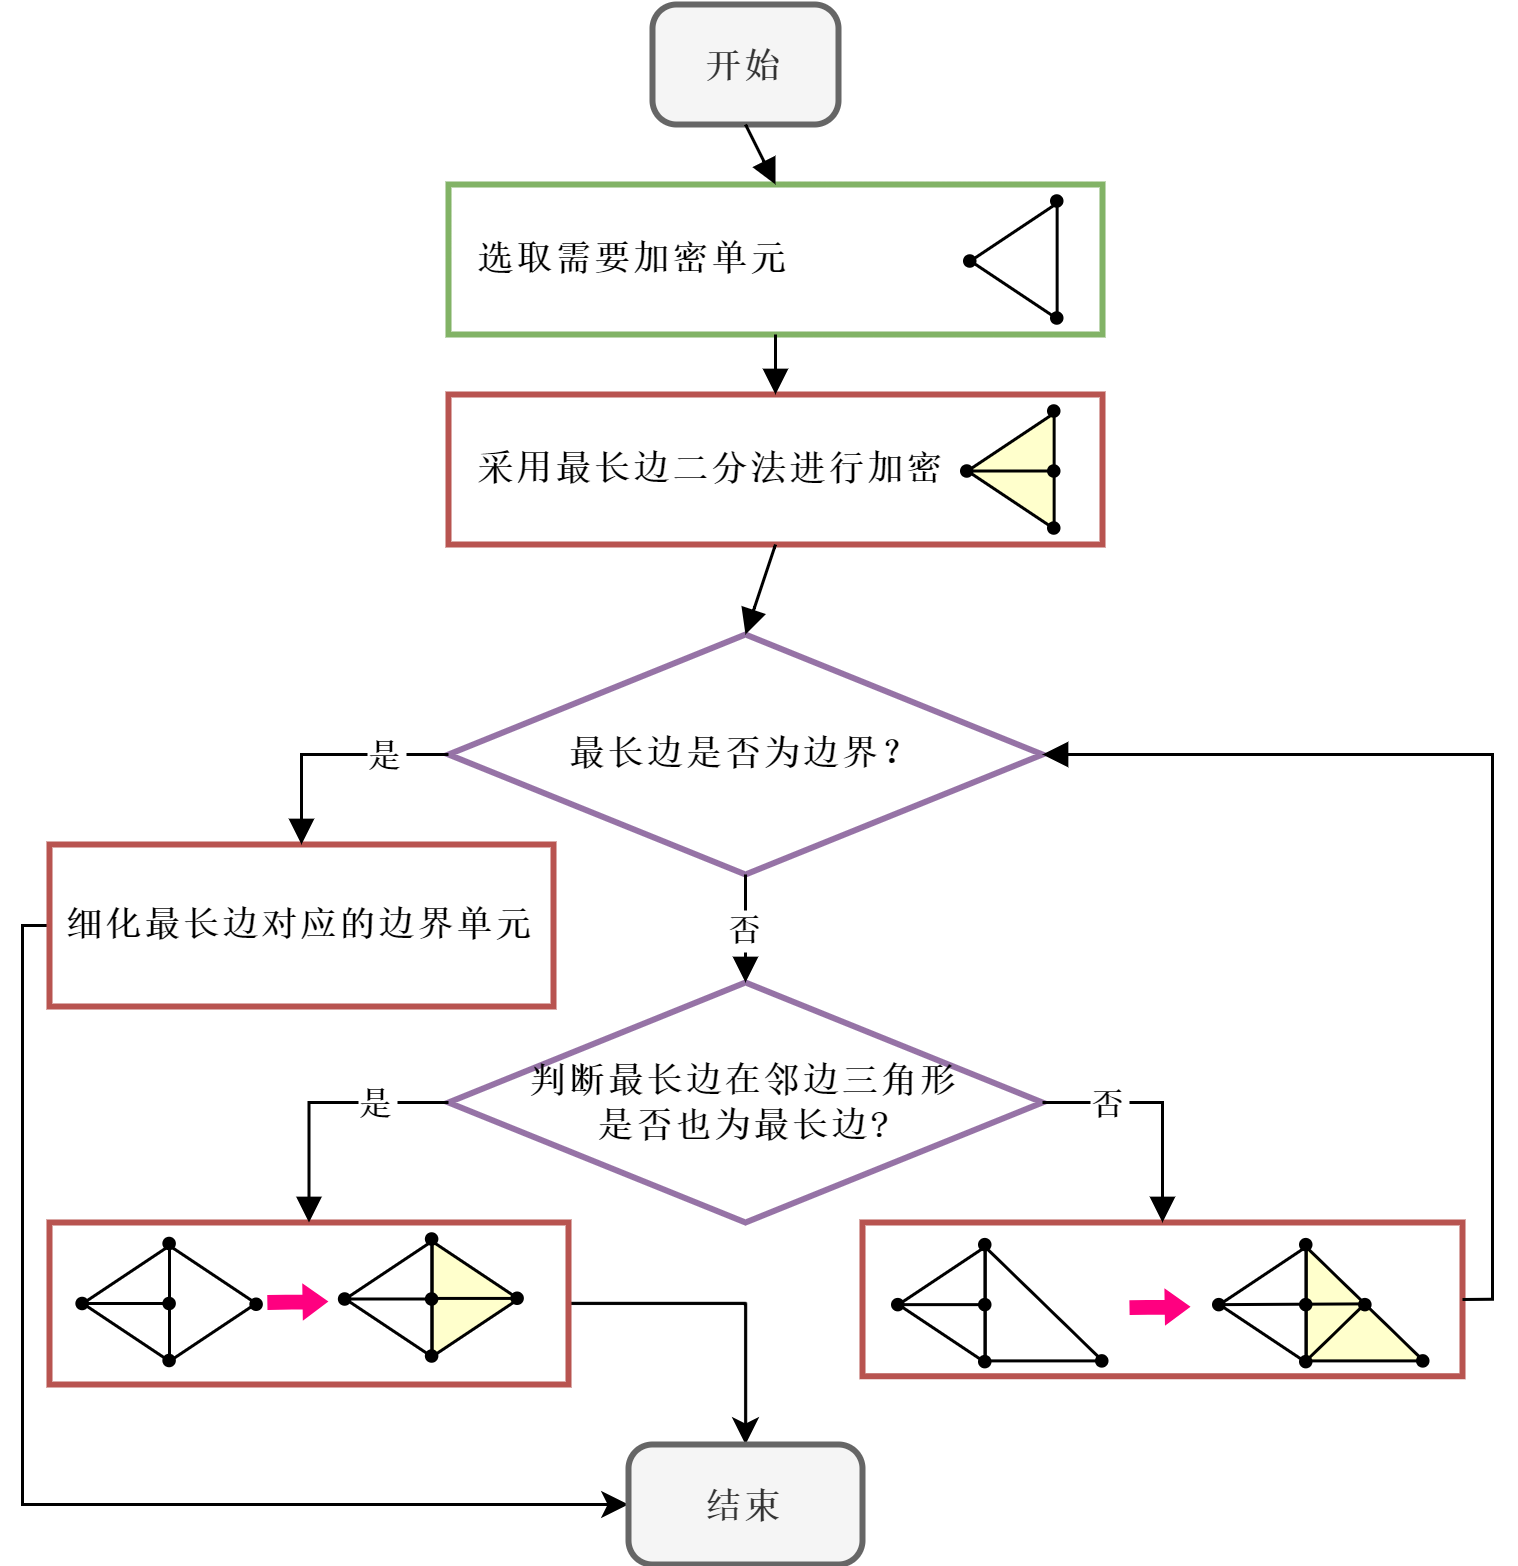
\includegraphics[scale=0.65]{fig/birefine.png}
\caption{\centering{半规则化网格演化流程图}}
\label{fg:Biliucheng}
\end{figure}

该网格局部细化的具体算法流程如图\ref{fg:Biliucheng}所示。
其核心思想是基于最长边二分法(Longest Edge Bisection)来协调相邻单元，
从而消除悬挂节点并保证网格的整体协调性。具体步骤如下：
首先，选取需要加密的目标三角形单元；
随后，对其采用最长边二分法进行临时加密，并首先判断该最长边是否为求解域的全局边界。
若是边界，则直接细化该最长边对应的边界单元并结束当前判定；
若该最长边并非边界，则进一步判断这条最长边是否同时也是其相邻三角形的最长边。
若是，则直接将这两个共边的相邻三角形沿着该最长边同步一分为二，完成加密并结束判定；
若该共用边不是相邻三角形的最长边，那么在二分当前单元后，
会在相邻单元的边上产生悬挂节点。此时需要将加密指令向相邻单元传递，
并对该相邻单元重新进入“最长边是否为边界”的系统判定与细分流程。
如此递归循环，直至所有由于局部细化产生的悬挂节点均被完美消除闭合。

基于上述最长边二分的协调加密机制，我们对该一维波动问题进行了多级网格演化。
首先构筑出全局的半规则化背景基础网格(BiRefine 无加密)；
随后精准定位预估误差带区域进行第1次局部网格细分(1次 Refine)，让特征区域内的三角形单元变得密集；
接着在上一级的基础上进一步缩小加密带宽度，进行第2次迭代加密(2次 Refine)；
最后收缩至核心梯度变化带完成第3次高度细分加密(3次 Refine)。
通过上述连续细分的四个阶段，我们在保留全局计算效率的前提下，
构建出了一条高度密集的局部网格带，用来更精确地捕获波前特征。

\subsection{一维弹性杆撞击刚性墙问题}

考虑一维弹性杆撞击刚性墙的问题，如图\ref{fg:impact_bar}所示，弹性杆的材料参数均取为单位值，即弹性模量 $E=1$，材料密度 $\rho=1$，杆总长 $L=1$。
在初始时刻，弹性杆整体具有向着刚性墙撞击的均匀初始速度 $v_0=1$。在撞击发生时，杆的左端受到刚性墙的阻挡，因此在该处施加强制的零位移边界条件：在任意时刻均始终满足 $u(0,t)=0$。同时，杆的右端不受外力约束，作为自由端施加自然边界条件。
由于杆的一端固定，另一端以均匀初速度运动，因此在这个一维波动问题中，杆内将会产生一个不断传播的压缩应力波。

\begin{figure}[!htb]
    \centering
    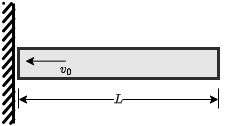
\includegraphics[width=0.6\textwidth]{fig/1.png}
    \caption{一维弹性杆撞击刚性墙示意图}
    \label{fg:impact_bar}
\end{figure}

为了验证算法的鲁棒性，
本文分别采用不同疏密度的三节点(Tri3)和六节点(Tri6)的三角形单元均布网格图\ref{fg:pengzhuangTri3wangge}进行离散。
图\ref{fg:pengzhuangTri3}和图\ref{fg:pengzhuangTri6}分别展示了一维弹性杆撞击刚性墙问题中，
在时空域上采用不同网格下的采用拉格朗日乘子时空混合离散有限元法数值计算的应力云图。

\begin{figure}[H]
    \centering
        \begin{tabular}{cccc}
            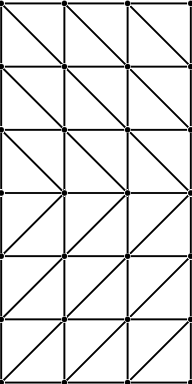
\includegraphics[width=0.2\textwidth]{fig/Tri3_b=2_4.png} &
            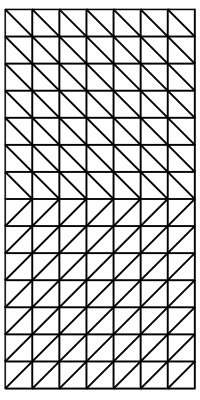
\includegraphics[width=0.2\textwidth]{fig/Tri3_b=2_8.png} &
            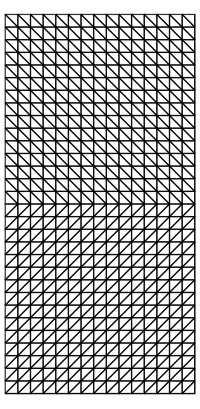
\includegraphics[width=0.2\textwidth]{fig/Tri3_b=2_16.png} &
            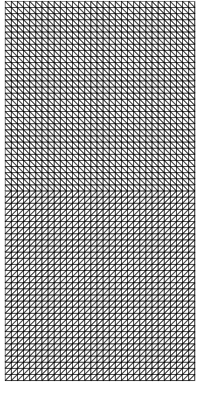
\includegraphics[width=0.2\textwidth]{fig/Tri3_b=2_32.png} \\
            $4\times8$ & $8\times16$ & $16\times32$ &  $32\times64$ \\
        \end{tabular}
        \caption{Tri3均布网格弹性杆问题不同密度下的节点模型}
        \label{fg:pengzhuangTri3wangge}
\end{figure}


从计算结果中可以明显看出，
采用基于拉格朗日变分方案的数值分析方法在时空域上求解弹性动力学问题时，
不仅计算过程简明（只需按照均布网格进行离散），而且计算效果优异。
不论是三节点三角形网格还是六节点三角形网格，都可以获得稳定的数值求解空间，
这表明该方法具有较好的精度适应性；且随着时间推移求解也不会产生明显的寄生振荡，
从而有效地提高了求解过程的稳定性和计算精度。
FIXME:加网格，颜色淡。加对比，换colormap.
\begin{figure}[H]
    \centering
        \begin{tabular}{cccc}
            
\includegraphics[width=0.2\textwidth]{fig/Tri3_4.png} &
            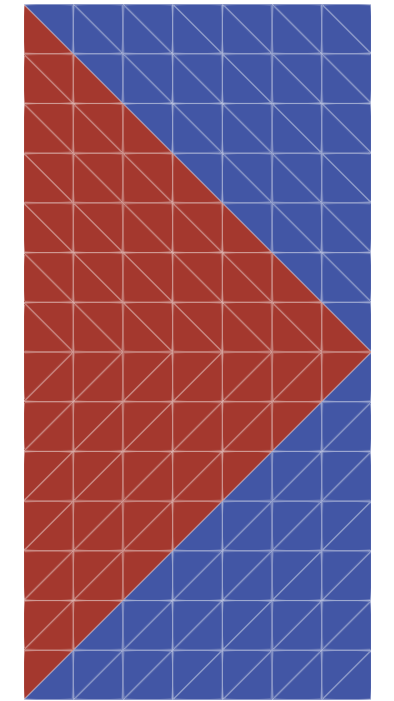
\includegraphics[width=0.2\textwidth]{fig/Tri3_8.png} &
            
\includegraphics[width=0.2\textwidth]{fig/Tri3_16.png} &
            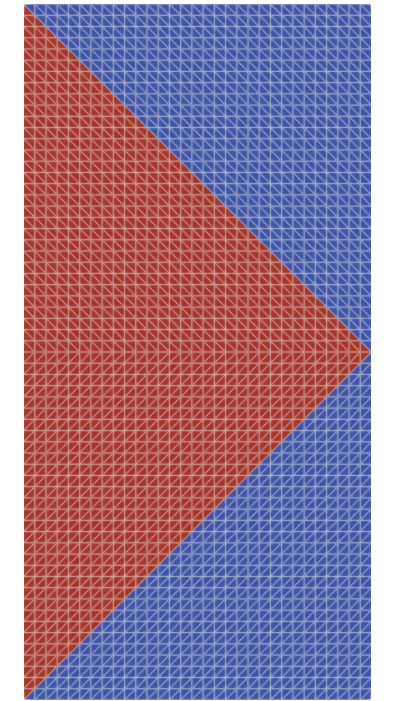
\includegraphics[width=0.2\textwidth]{fig/Tri3_32.png}\makebox[0pt][l]{\hspace{5pt}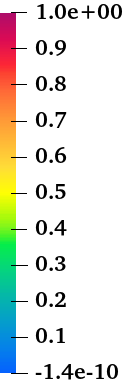
\includegraphics[width=0.1\textwidth]{fig/legend.png}} \\
            $4\times8$ & $8\times16$ & $16\times32$ &  $32\times64$ \\
        \end{tabular}
        \caption{Tri3均布网格弹性杆问题不同密度下的应力云图}
        \label{fg:pengzhuangTri3}
\end{figure}

\begin{figure}[H]
    \centering
        \begin{tabular}{cccc}
            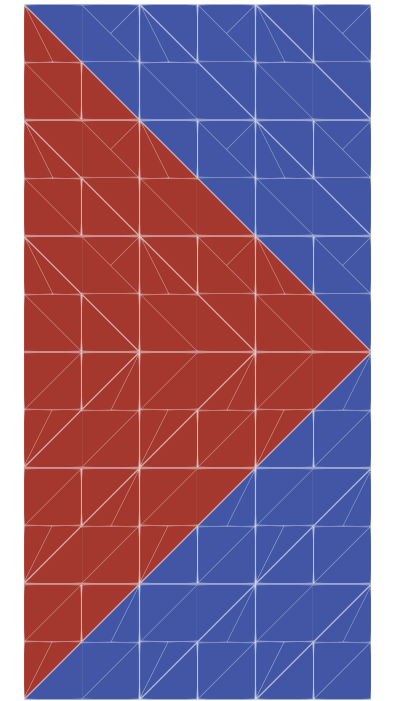
\includegraphics[width=0.2\textwidth]{fig/Tri6_4.png} &
            
\includegraphics[width=0.2\textwidth]{fig/Tri6_8.png} &
            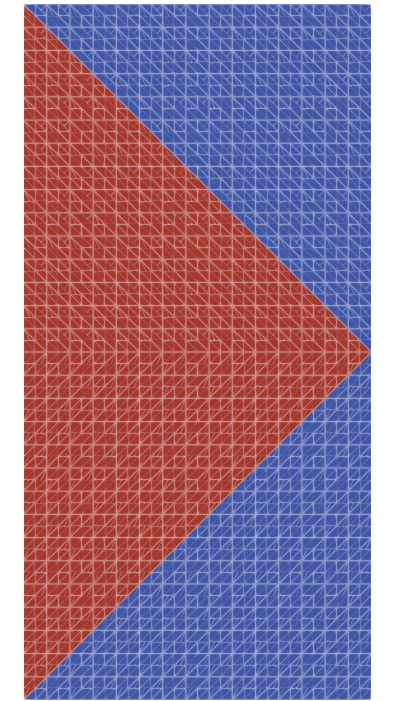
\includegraphics[width=0.2\textwidth]{fig/Tri6_16.png} &
            
\includegraphics[width=0.2\textwidth]{fig/Tri6_32.png}\makebox[0pt][l]{\hspace{5pt}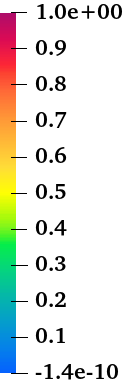
\includegraphics[width=0.1\textwidth]{fig/legend.png}} \\
            $4\times8$ & $8\times16$ & $16\times32$ &  $32\times64$ \\
        \end{tabular}
        \caption{Tri6均布网格弹性杆问题不同密度下的节点模型以及应力云图}
        \label{fg:pengzhuangTri6}
\end{figure}
 









\subsection{一维弹性材料层中的波动问题}
考虑一个厚度为$H=4$的弹性材料层，如图\ref{fg:tension_bar}所示，材料密度$\rho = 1$,弹性模量$E = 1$，波速$\alpha = 1$。
在材料的右侧边界施加位移等于零的强制边界条件。
当$t = 0$时，在材料左边界施加一个持续时间为$1$的压缩应力脉冲$T$，
压缩应力脉冲$T$的示意图为图\ref{fg:impulse wave},表达式为：
FIXME T换P
\begin{equation}
    T_{11}(0,t)=\begin{cases}
    -\sin(\pi t),& 0\leq t\leq 1,\\
    0,              & 1 < t.
    \end{cases}
\end{equation}

\begin{figure}[!h]
    \centering
    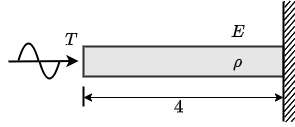
\includegraphics[scale=0.7]{fig/2.png}
\caption{\centering{一维弹性材料层中的波动问题示意图}}
\label{fg:tension_bar}
\end{figure}

\begin{figure}[!h]
    \centering
    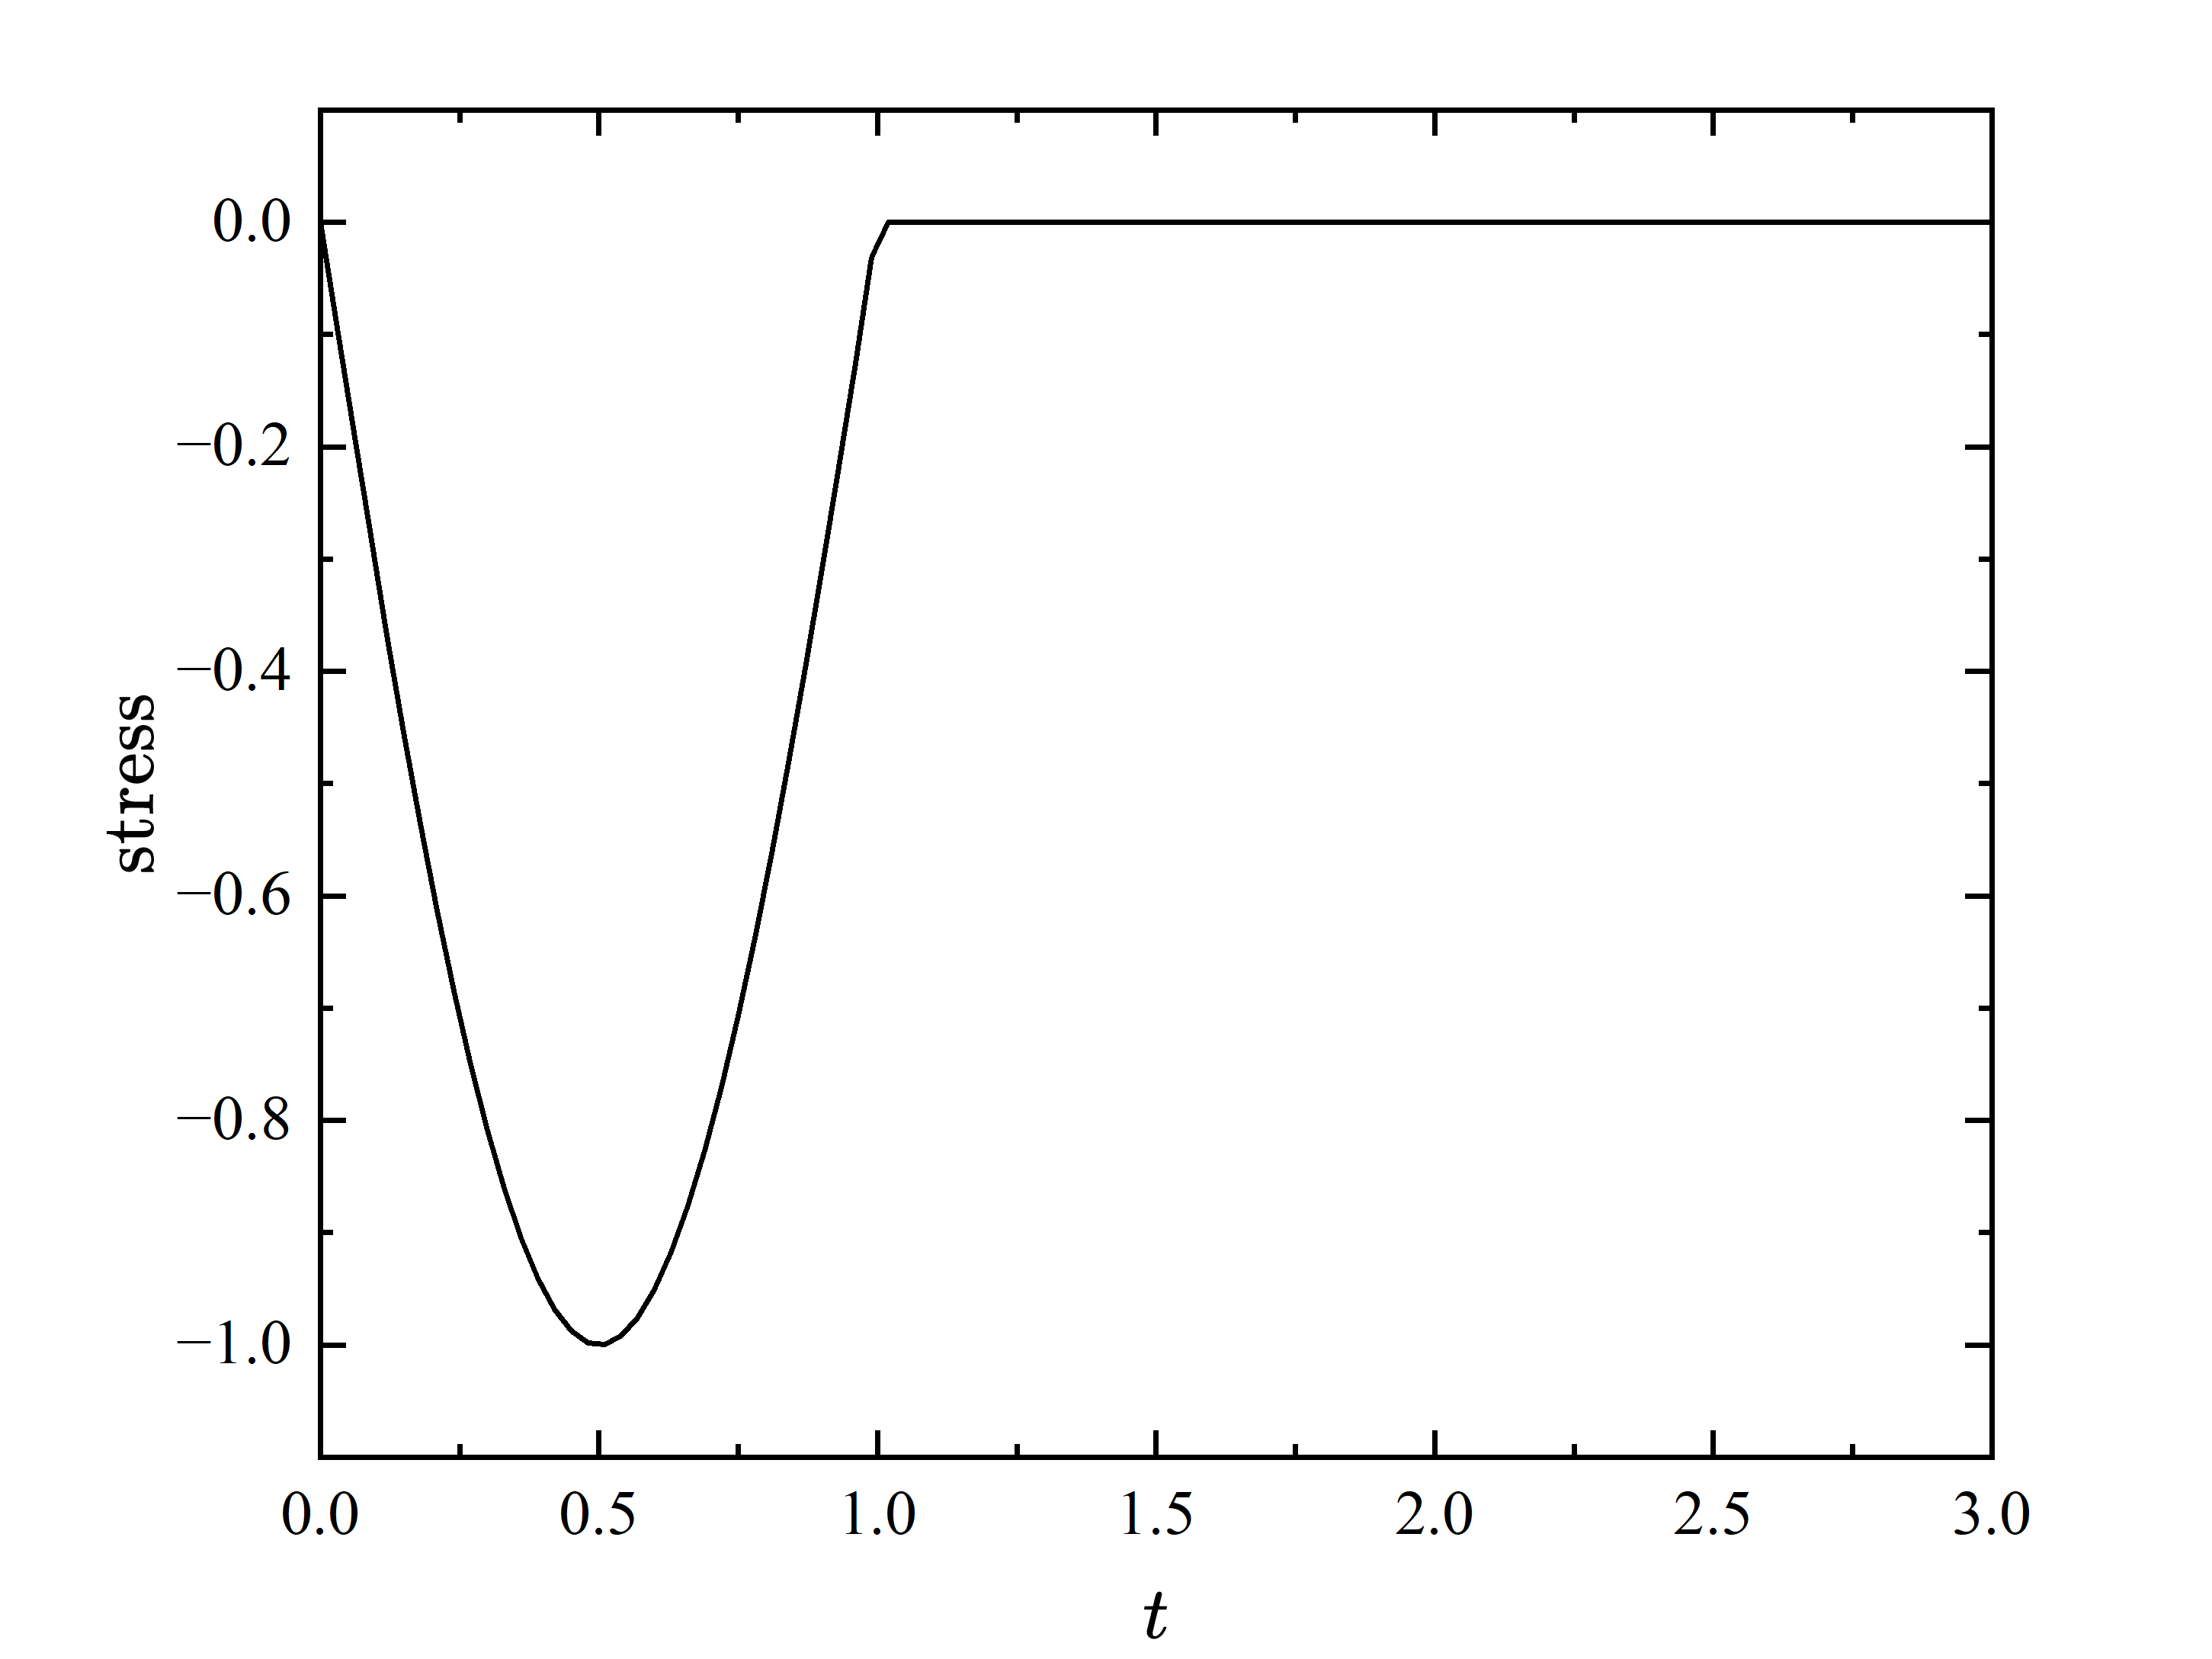
\includegraphics[scale=0.4]{fig/脉冲图.png}
\caption{\centering{施加在弹性材料左侧的应力}}
\label{fg:impulse wave}
\end{figure}

在此脉冲边界条件的影响下，位移的精确解的解析表达式为：
\begin{equation}
  u_1(x_1,t)=
    \begin{cases}
      \frac{2\alpha}{\pi}, & x_1 < \alpha(t - 1),\\
      \frac{\alpha}{\pi}\left[1 - \cos\left(\pi\left(t - \frac{x_1}{\alpha}\right)\right)\right], & \alpha(t - 1) \leq x_1 \leq \alpha t,\\
       0, & \alpha t < x_1.
    \end{cases}
\end{equation}

\begin{figure}[!h]
    \centering
        \begin{tabular}{c@{\hspace{20pt}}c}
            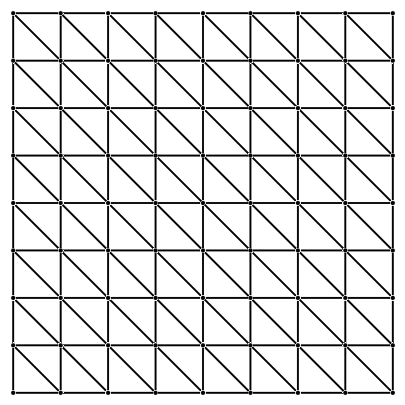
\includegraphics[width=0.3\textwidth]{fig/Tri3_square_8.png} &
            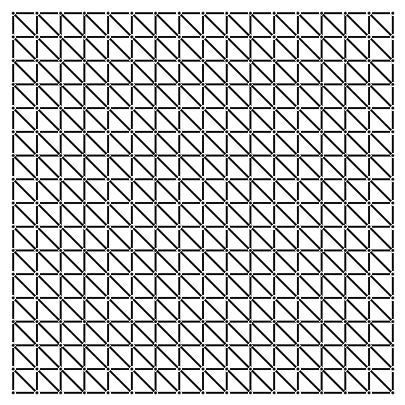
\includegraphics[width=0.3\textwidth]{fig/Tri3_square_16.png} \\
            $9\times9$ & $17\times17$ \\
            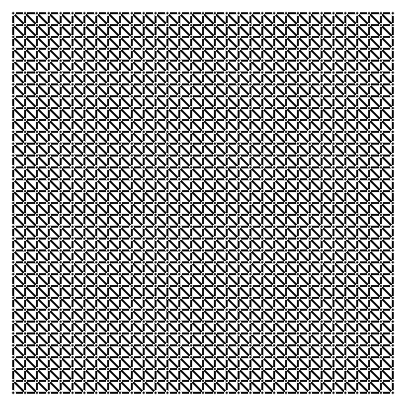
\includegraphics[width=0.3\textwidth]{fig/Tri3_square_32.png} &
            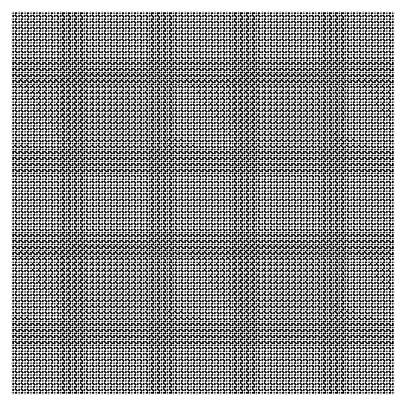
\includegraphics[width=0.3\textwidth]{fig/Tri3_square_64.png} \\
            $33\times33$ & $65\times65$ \\
        \end{tabular}
        \caption{弹性材料波动问题节点模型}\label{fg:square node model}
\end{figure}

弹性材料的求解域分别通过图\ref{fg:square node model}所示采用均布的四个疏密不同、
三节点三角形单元网格进行离散。
图\ref{fg:ecr}为采用上述四个疏密不同的离散节点时的位移误差和能量误差的收敛结果。
从图中可以看出采用基于
拉格朗日变分方案的数值分析方法在时空域上求解弹性材料波动问题时， 
位移误差收敛率为$2.0$，能量误差收敛率为$1.0$，
其位移误差和能量误差均能达到理论收敛率。
\begin{figure}[!h]
    \centering
    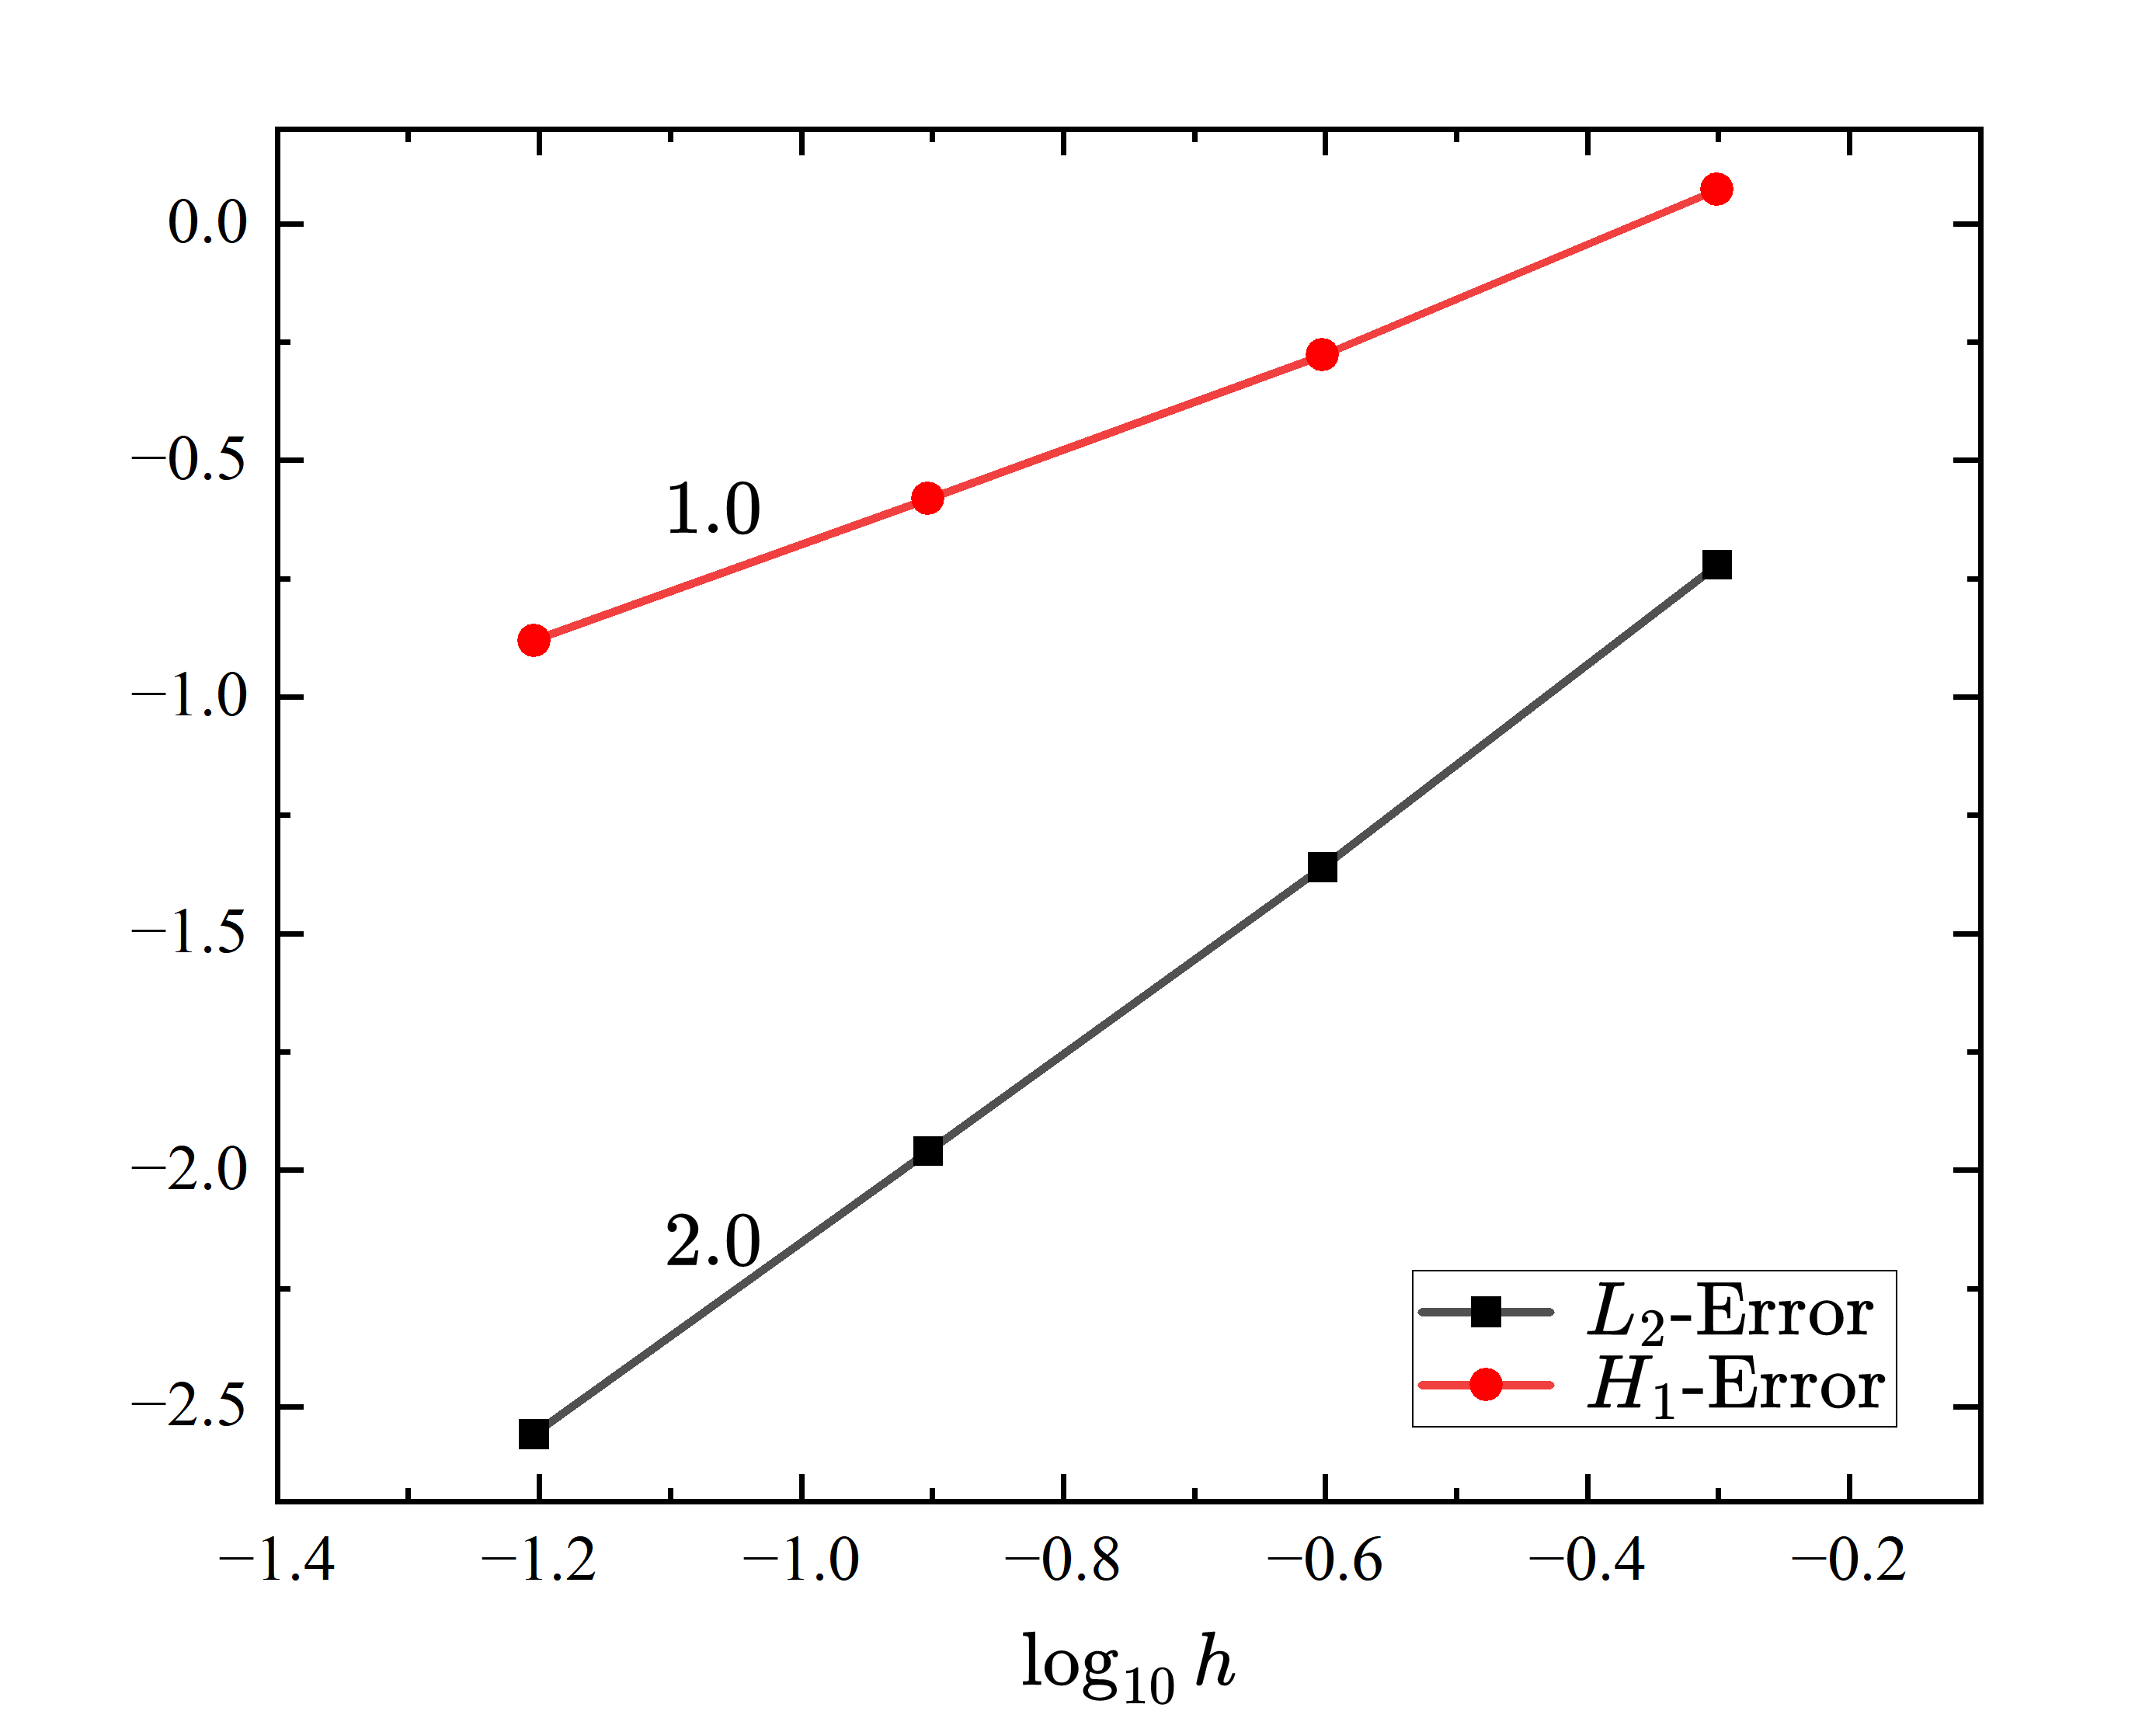
\includegraphics[scale=0.38]{fig/Tri3均布误差收敛率.png}
\caption{\centering{一维弹性材料波动问题采用Tri3单元计算的误差收敛结果}}
\label{fg:ecr}
\end{figure}

同样，当我们采用六节点单元以相同的疏密程度去计算一维弹性材料层中的波动问题时，
最终得到的计算结果如图\ref{fg:Hecr}所示，位移误差收敛率和能量误差收敛率均能达到理论误差收敛率。
\begin{figure}[!h]
    \centering
    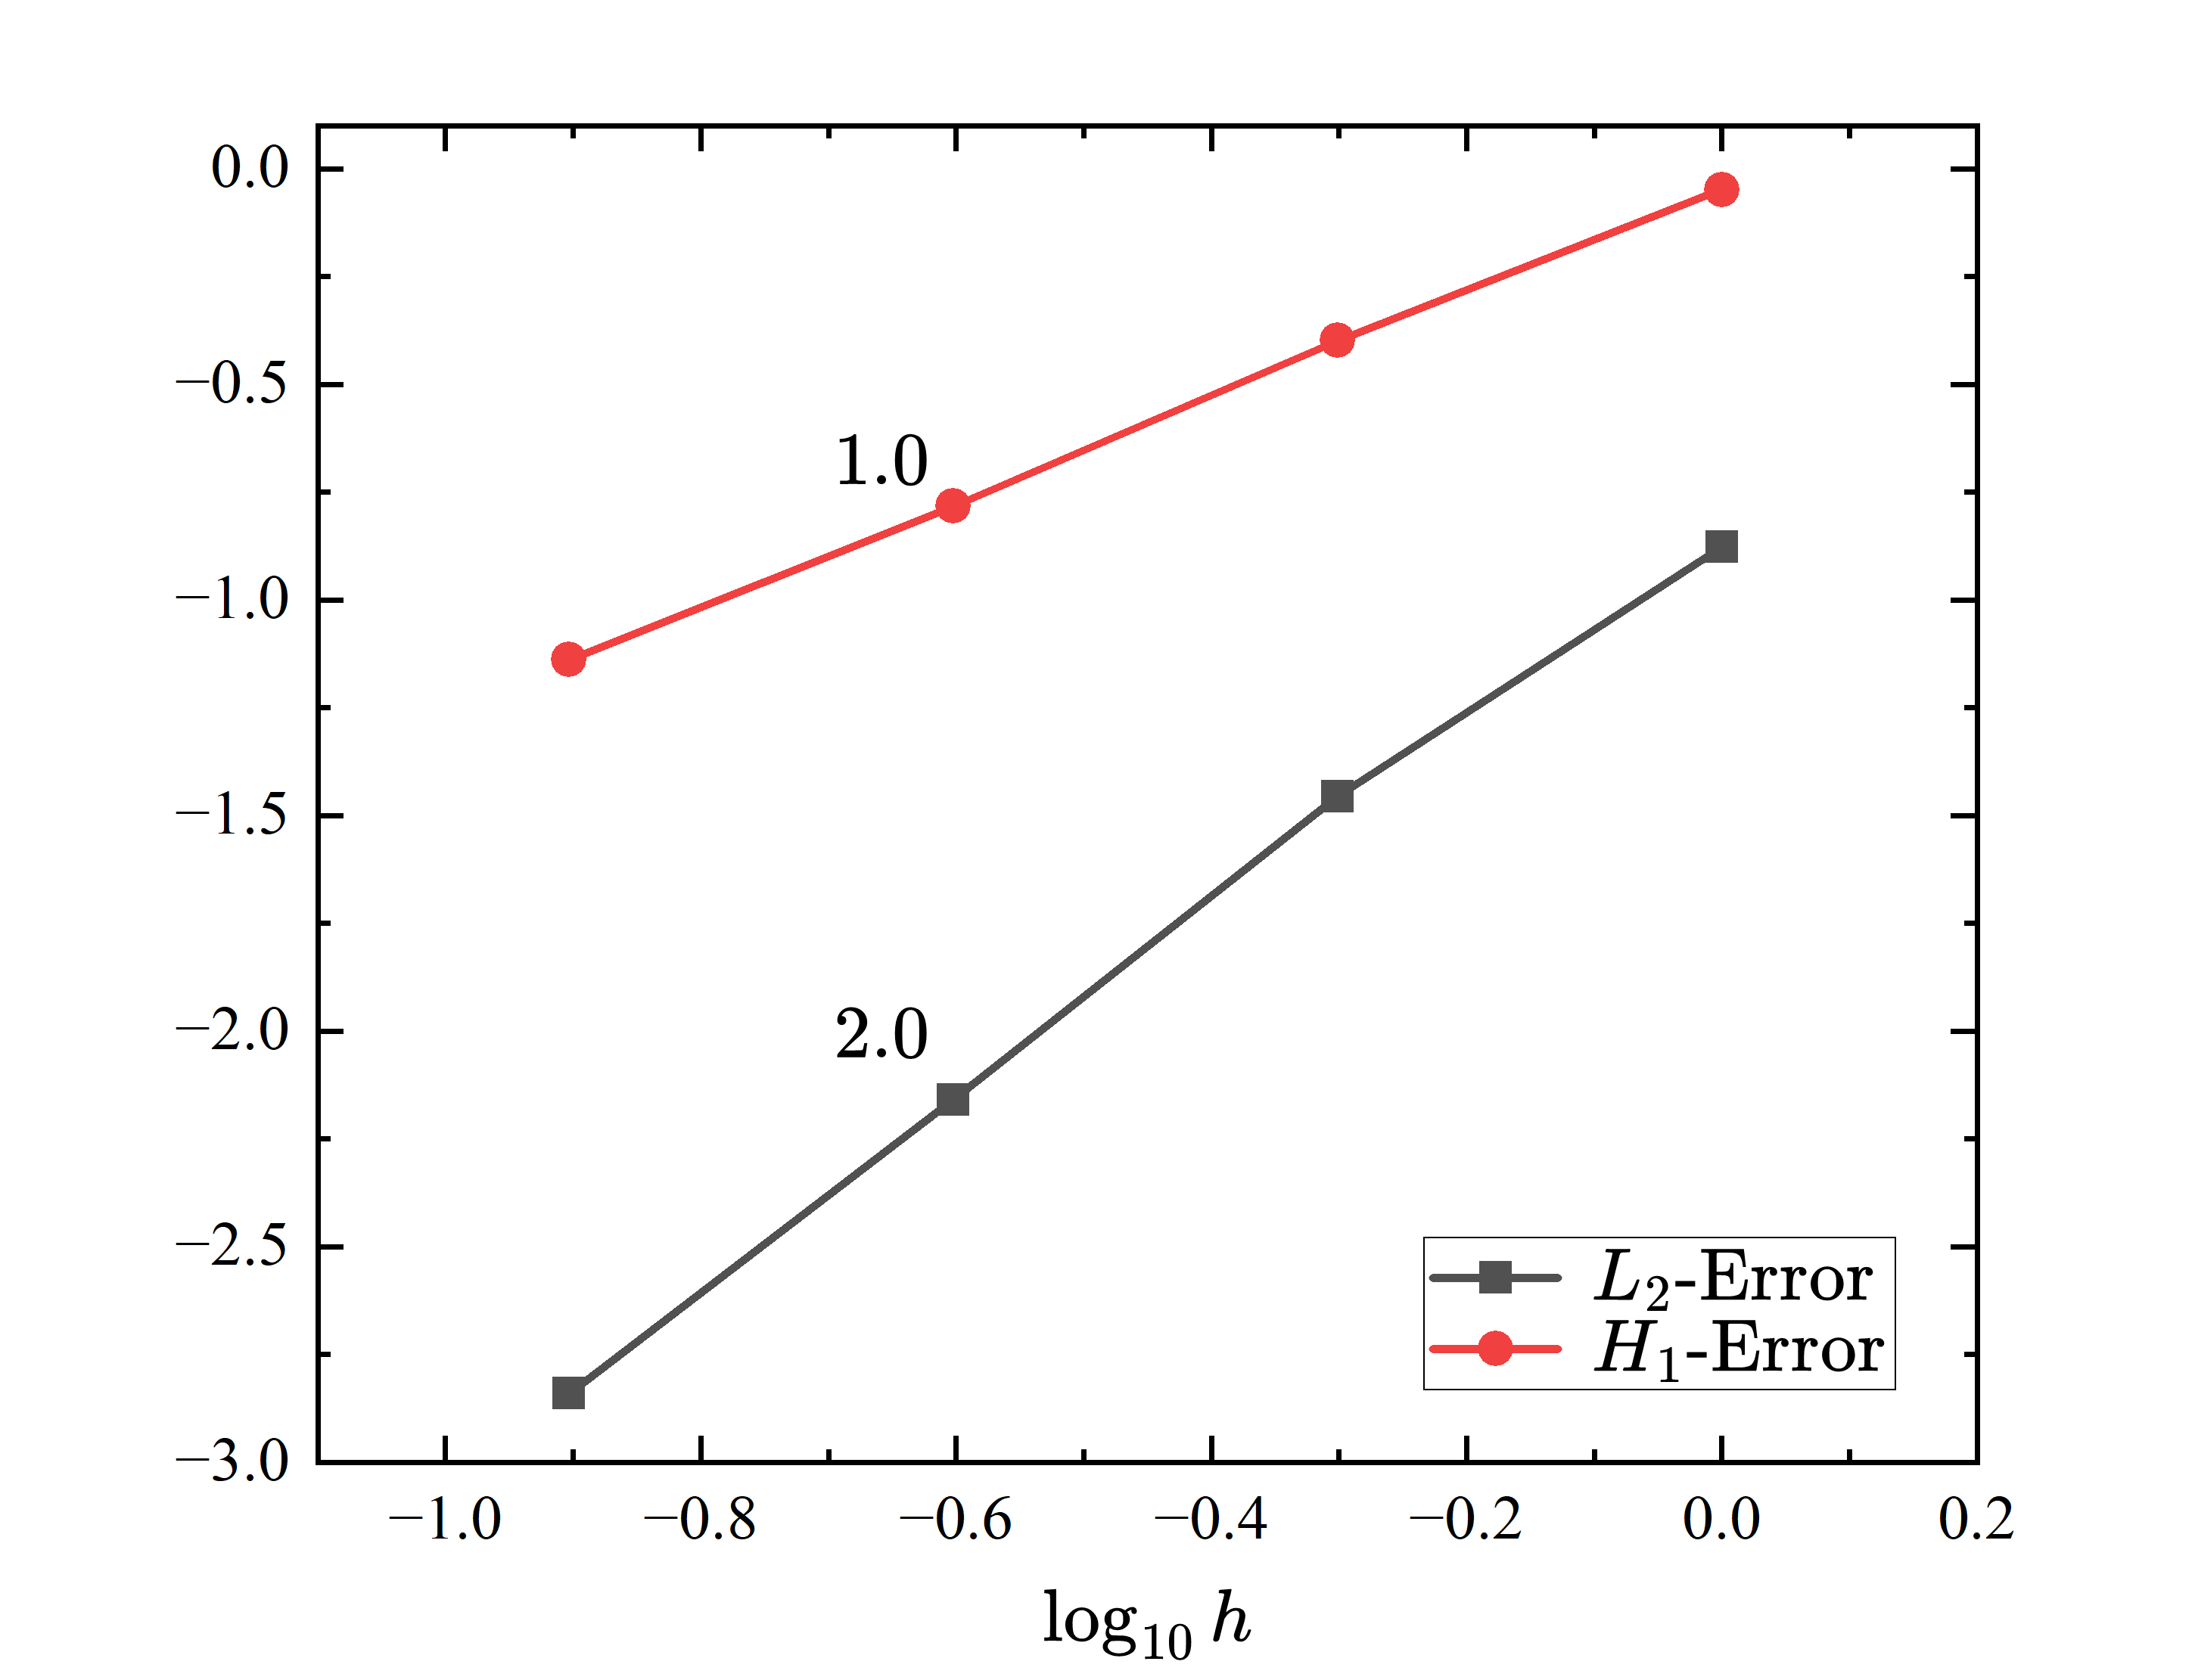
\includegraphics[scale=0.38]{fig/Tri6_(4-32).png}
\caption{\centering{一维弹性材料波动问题采用Tri6单元计算的误差收敛结果}}
\label{fg:Hecr}
\end{figure}

一维弹性材料波动问题在非均布的网格节点上进行计算时会产生较大的振荡现象，
为解决这一问题，尝试对梯度进行改变的区域做局部加密进行计算，
对非均布网格适当的局部加密。
如图\ref{fg:local}所示，对20*20的非均布网格在解的坡顶进行局部加密，
来缓解梯度变化带来的振荡现象，从而得到更加稳定的数值解。
\begin{figure}[H]
    \centering
        \begin{tabular}{c@{\hspace{20pt}}c}
            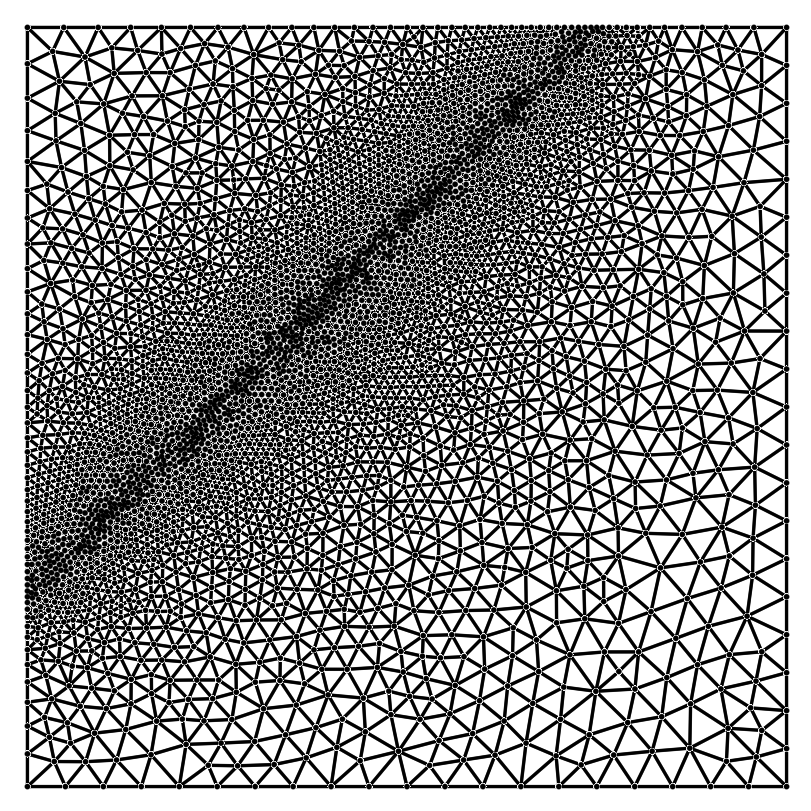
\includegraphics[width=0.4\textwidth]{fig/Tri3非均布_Jbjm_0.03.png} &
            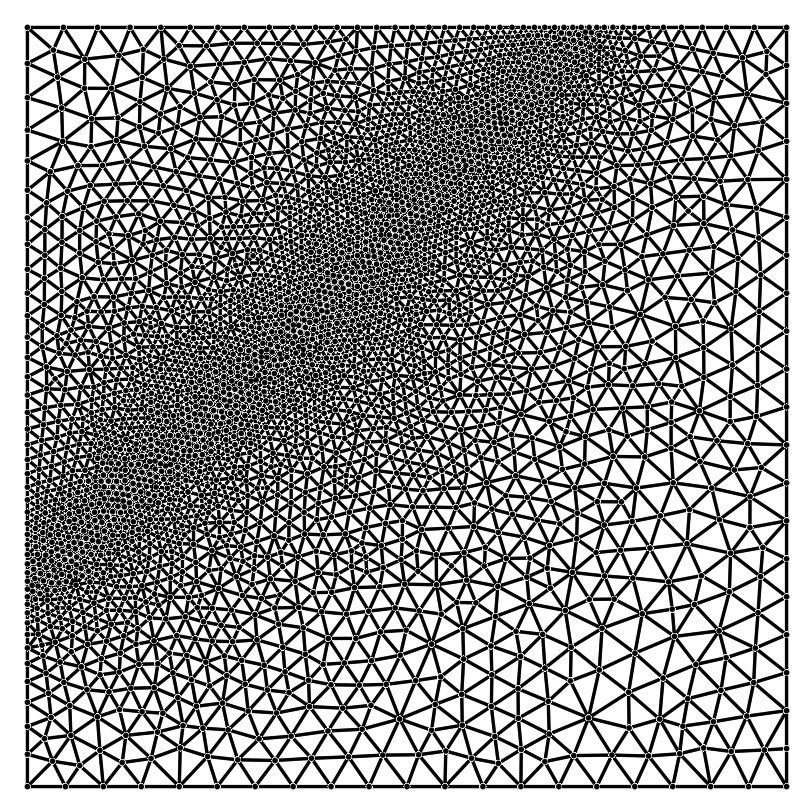
\includegraphics[width=0.4\textwidth]{fig/Tri3非均布_Jbjm_0.04.png} \\
            $c=0.03$网格示意图 & $c=0.04$网格示意图  \\
            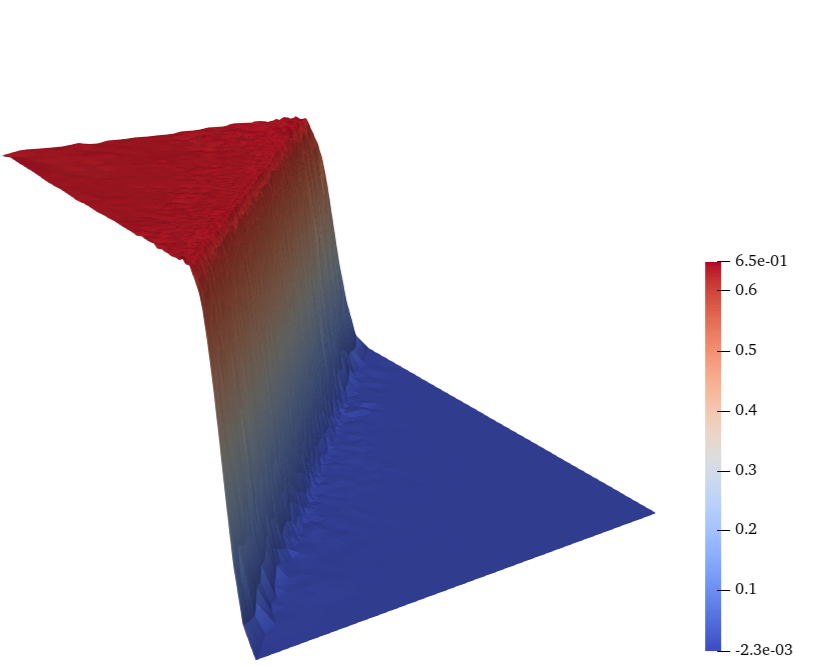
\includegraphics[width=0.5\textwidth]{fig/C=0.2_c=0.03.png} &
            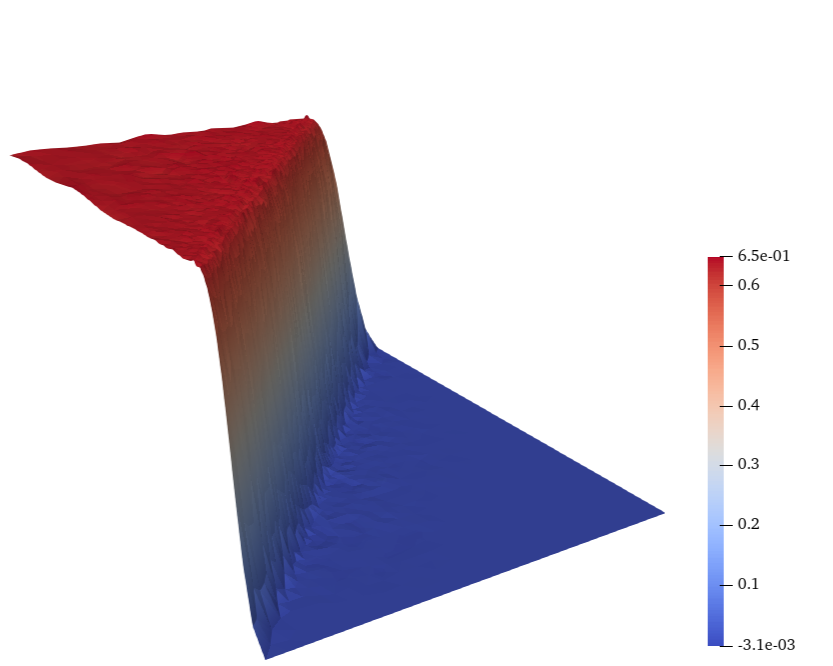
\includegraphics[width=0.5\textwidth]{fig/C=0.2_c=0.04.png} \\
            $c=0.03$位移图 & $c=0.04$位移图 \\
        \end{tabular}
        \caption{弹性材料波动问题局部加密计算的三维位移图}\label{fg:local}
\end{figure}


完整的网格生成演化图如下：
 
\begin{figure}[H]
    \centering
        \begin{tabular}{c@{\hspace{20pt}}c}
            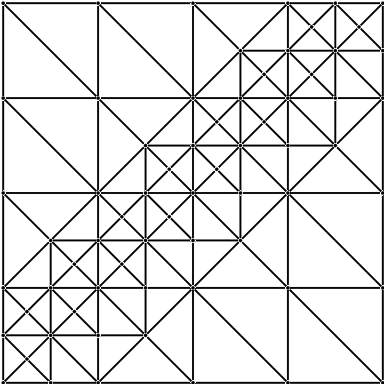
\includegraphics[width=0.3\textwidth]{fig/impact_4_refined_r10.png} &
            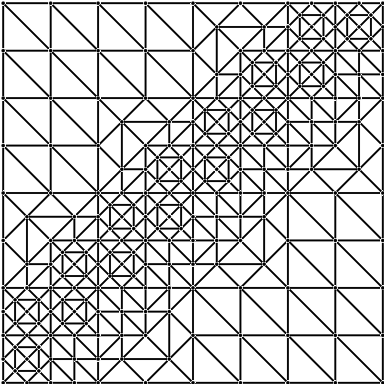
\includegraphics[width=0.3\textwidth]{fig/impact_4_refined_r11.png} \\
            BiRefine & 1次Refine \\[5pt]
            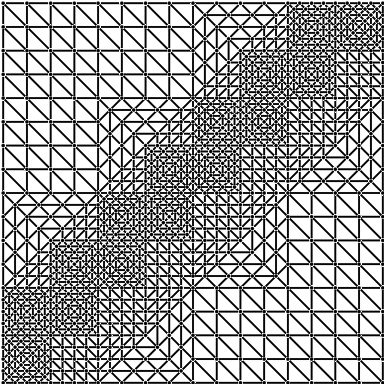
\includegraphics[width=0.3\textwidth]{fig/impact_4_refined_r12.png} &
            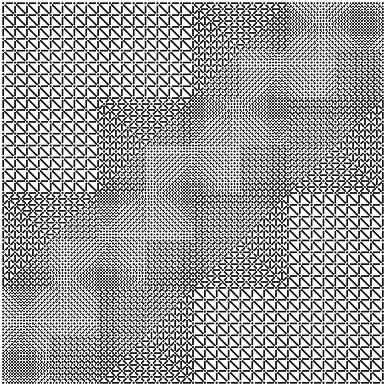
\includegraphics[width=0.3\textwidth]{fig/impact_4_refined_r13.png} \\
            2次Refine & 3次Refine \\
        \end{tabular}
        \vspace{-0.5em}
        \caption{弹性材料波动问题节点模型}\label{fg:Birefine}
\end{figure}

根据上述的BiRefine生成的网格进行离散计算，
图\ref{fg:BiL2H1}为采用上述四个疏密不同的离散节点时的位移误差和能量误差的收敛结果。
从图中可以看出采用基于拉格朗日变分方案的数值分析方法在时空域上求解弹性材料波动问题时，
其位移误差和能量误差均能达到理论收敛率。

\begin{figure}[H]
    \centering
    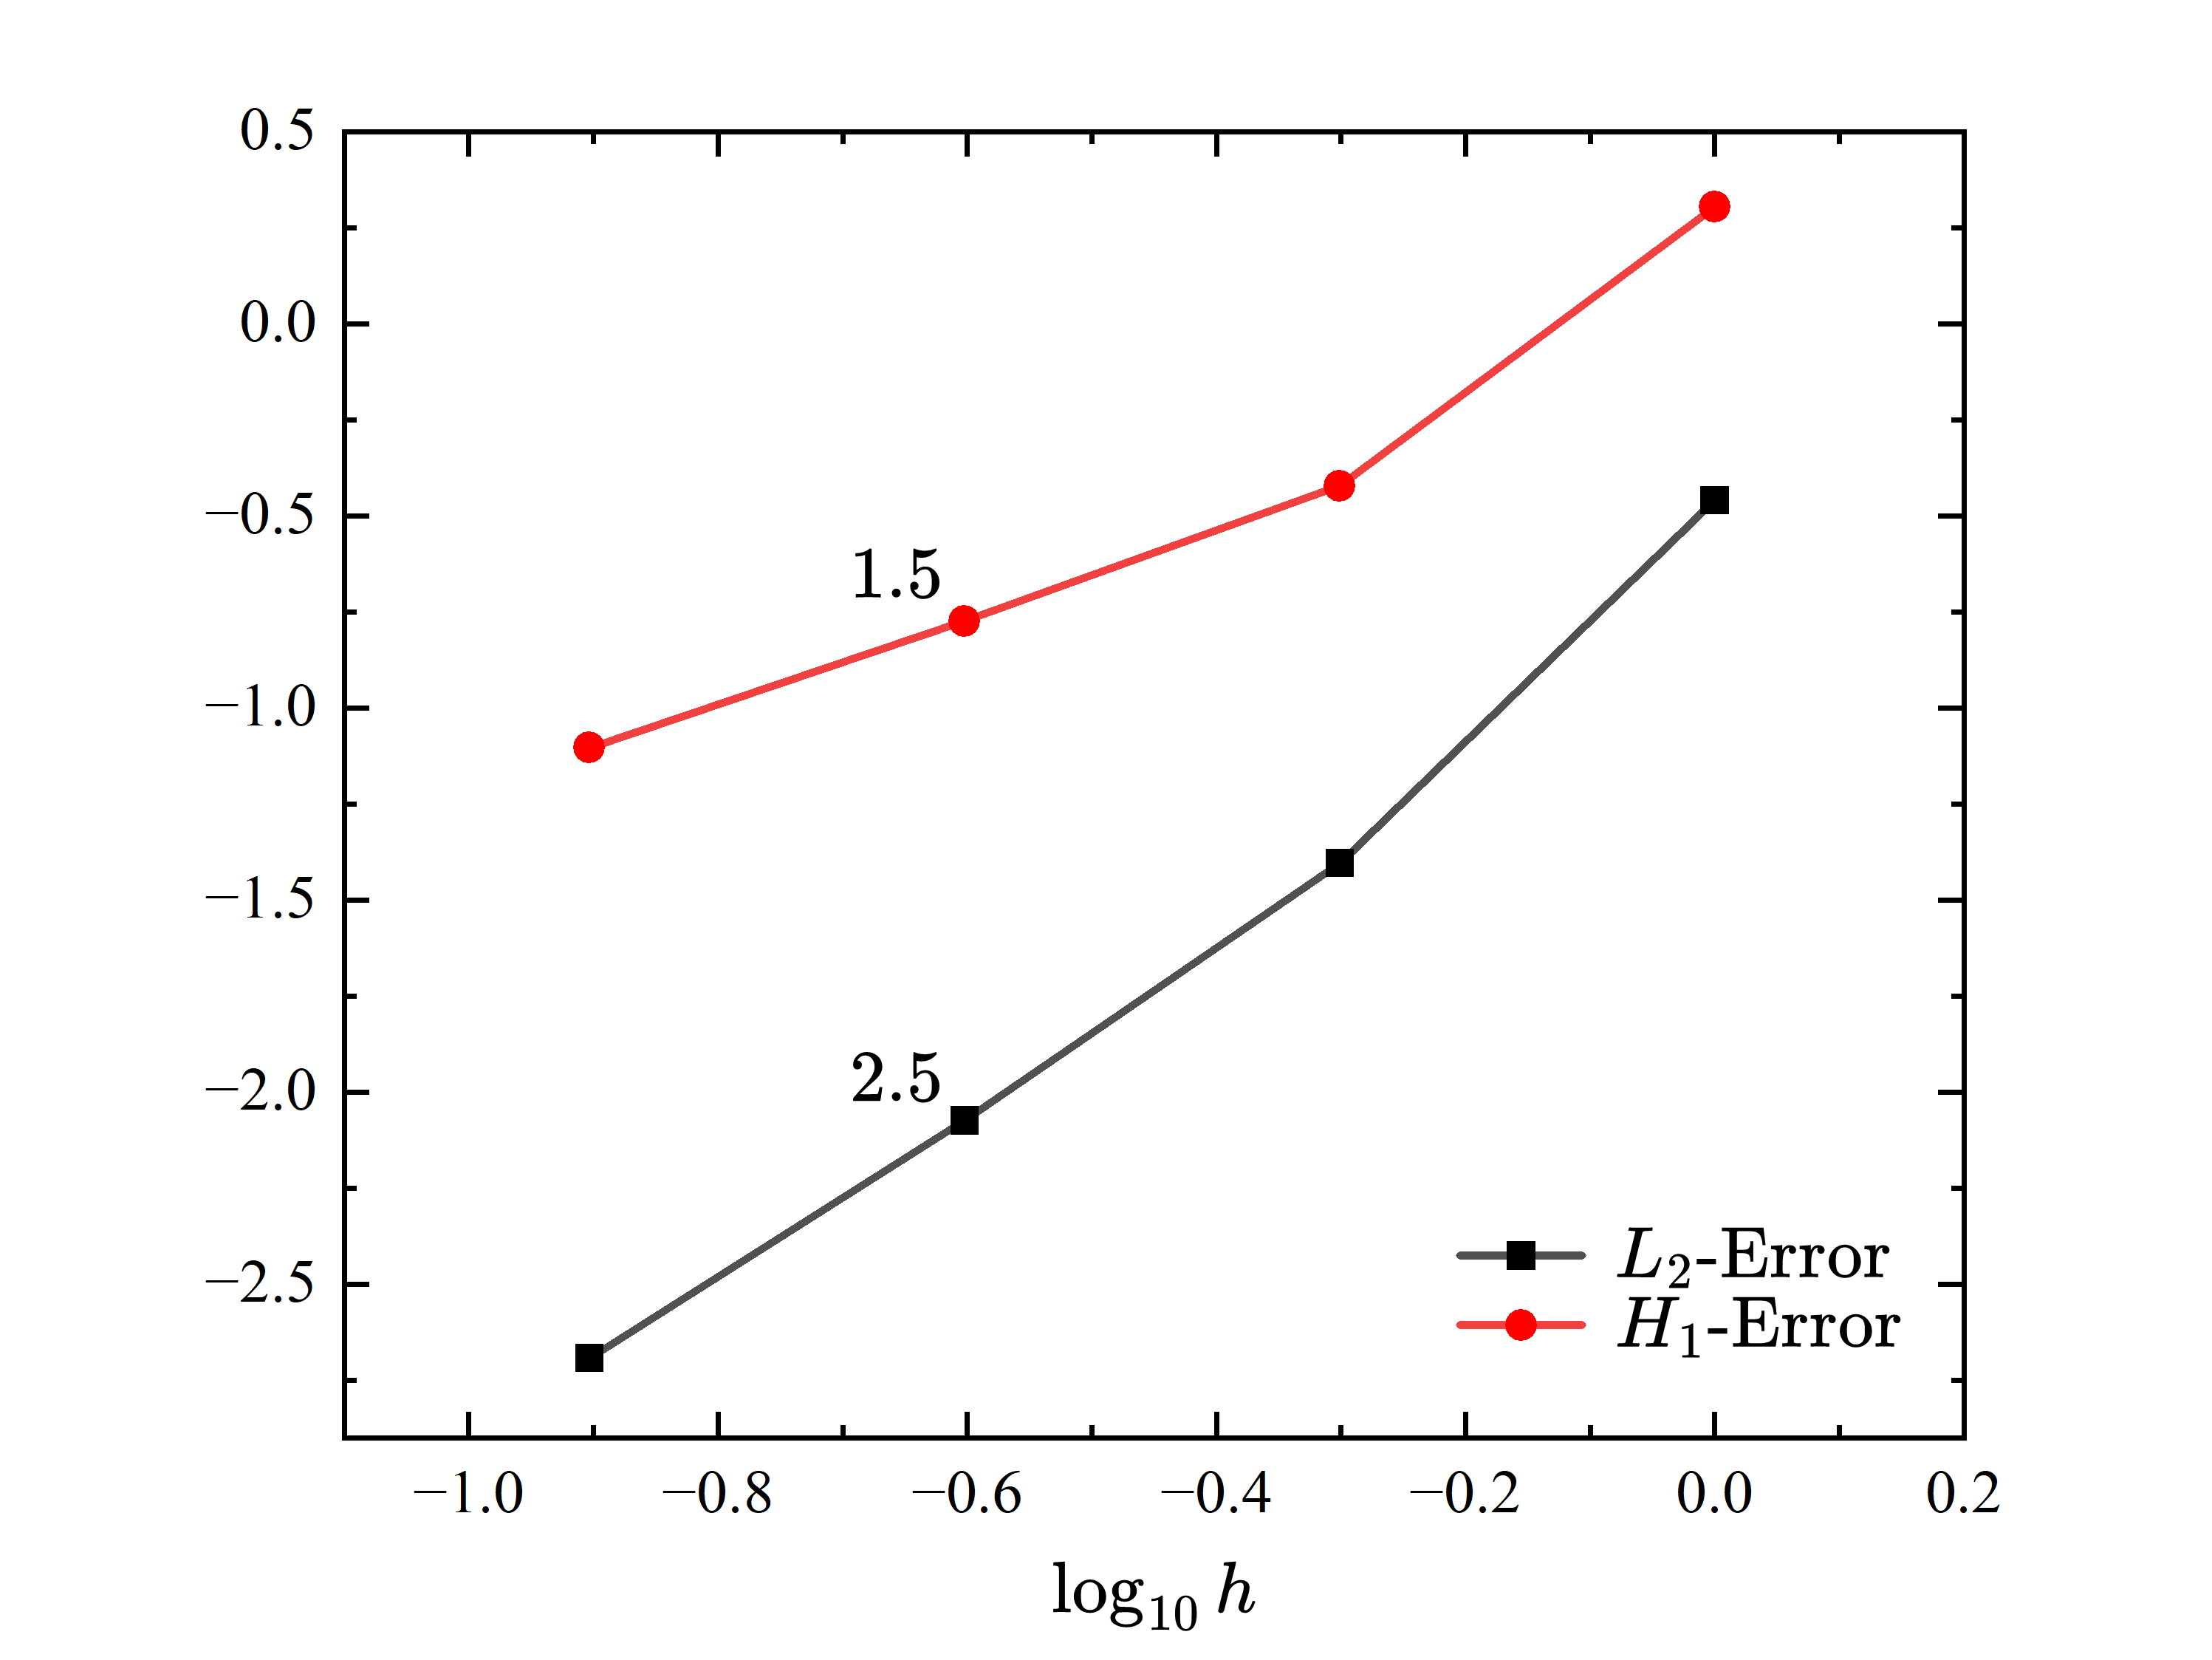
\includegraphics[scale=0.38]{fig/BiRefine_2d(r10-r13)_4-32.png}
\caption{\centering{一维弹性材料波动问题采用BiRefine单元计算的误差收敛结果}}
\label{fg:BiL2H1}
\end{figure}












\subsection{一维弦的横向自由振动问题}
考虑一根长度为$l$的均匀弦，两端固定，如图\ref{fg:xian}所示，
材料密度$\rho=1.0$，弹性模量$E=1.0$，波速$\alpha =1.0$，
在初始时刻具有一定的位移和速度，做自由横向振动。

\begin{figure}[!h]
    \centering
    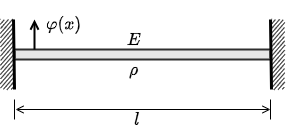
\includegraphics[scale=0.7]{fig/一维弦横向振动.png}
\caption{\centering{一维弦横向自由振动问题示意图}}
\label{fg:xian}
\end{figure}

弦的自由振动满足一维波动方程，结合边界条件和初始条件，问题可表述为：
\begin{equation}\label{3.3}
\left \{
\begin{split}
& u_{,tt} - \alpha^2 u_{xx} = 0 \\
& u(0,t) = u(l,t) = 0 \\
& u(x,0) = \varphi(x) , u_t(x,0) = \phi(x)
\end{split}
\right . 
\end{equation}

采用分离变量法将波动方程分解为常微分方程，
结合边界条件可得到波动方程的通解为：
\begin{equation}\label{3.4}
u(x,t) =  \sum_{n=1}^{\infty} [A_n \cos \frac{n\pi a}{l}t + B_n \sin \frac{n\pi a}{l}t ]\sin\frac{n\pi x}{l}
\end{equation}

简化方程，令$A = 1$，$B = 0$，$n = 1$得到精确解解析表达式：
\begin{equation}
u(x,t) =  \cos (\frac{\pi a}{l}t) \sin\frac{\pi x}{l}
\end{equation}

以及位移边界条件：
\begin{equation}\label{3.6}
\begin{split}
& u (x,0) = \sin \frac{\pi x}{l} = \varphi(x) \\
& u _t(x,0) = 0
\end{split}
\end{equation}

FIXME: 排版。空白太多。colorbar。
\begin{figure}[!h]
    \centering
        \begin{tabular}{c@{\hspace{20pt}}c}
            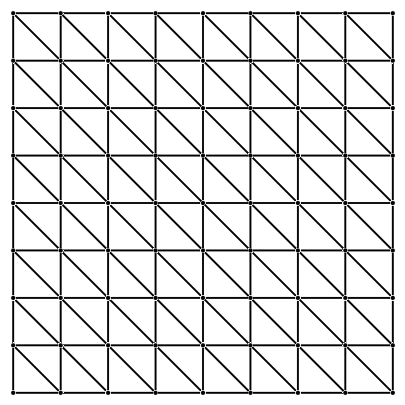
\includegraphics[width=0.3\textwidth]{fig/Tri3_square_8.png} &
            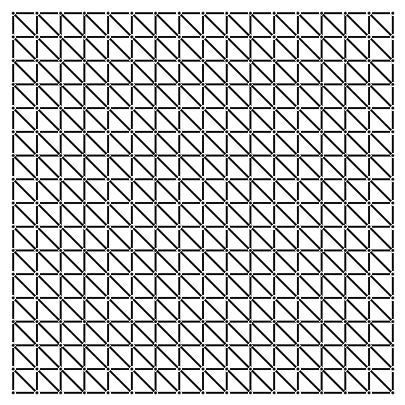
\includegraphics[width=0.3\textwidth]{fig/Tri3_square_16.png} \\
            $9\times9$ & $17\times17$ \\
            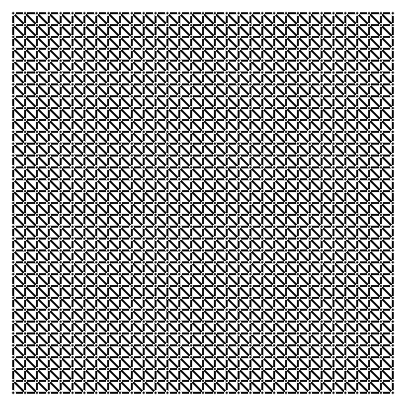
\includegraphics[width=0.3\textwidth]{fig/Tri3_square_32.png} &
            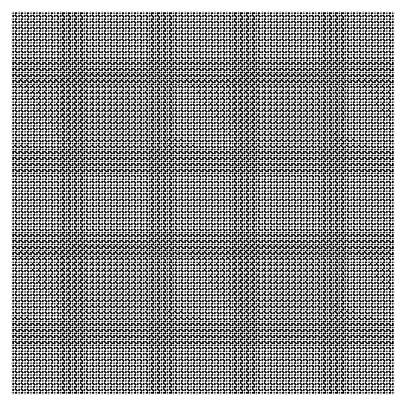
\includegraphics[width=0.3\textwidth]{fig/Tri3_square_64.png} \\
            $33\times33$ & $65\times65$ \\
        \end{tabular}
        \caption{一维弦自由横向振动问题三角形三节点单元模型}\label{fg:yiweixianwangge}
\end{figure}

\begin{figure}[!h]
    \centering
        \begin{tabular}{c@{\hspace{20pt}}c}
            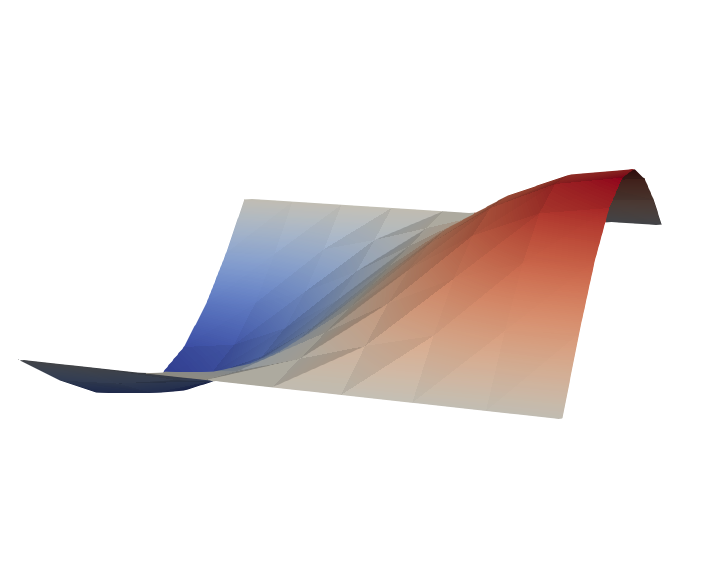
\includegraphics[width=0.4\textwidth]{fig/Tri3_uniform_8.png} &
            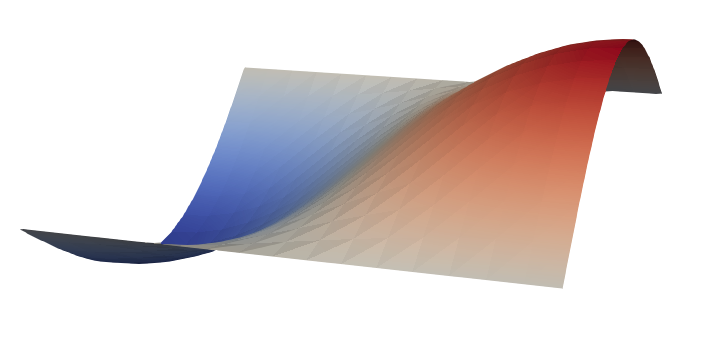
\includegraphics[width=0.4\textwidth]{fig/Tri3_uniform_16.png} \\
            $9\times9$ & $17\times17$ \\
            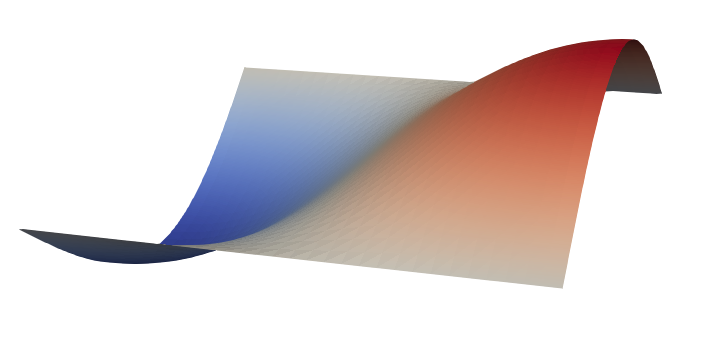
\includegraphics[width=0.4\textwidth]{fig/Tri3_uniform_32.png} &
            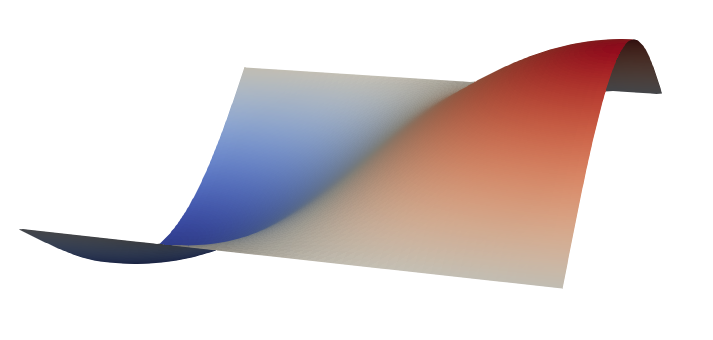
\includegraphics[width=0.4\textwidth]{fig/Tri3_uniform_64.png} \\
            $33\times33$ & $65\times65$ \\
        \end{tabular}
        \caption{一维弦自由横向振动问题三节点单元计算位移图}\label{fg:yiweixiansanjiedianweiyitu}
\end{figure}

一维弦自由横向振动问题的求解域也可以通过图\ref{fg:yiweixianwangge}所示，
采用均布的四个疏密不同、三节点三角形单元网格进行离散，在这个网格单元下，
当我们采用基于拉格朗日变分方案的完全弱形式伽辽金法去计算该问题时，
我们可以得到图\ref{fg:yiweixiansanjiedianweiyitu}所示的位移结果，
可以看出，无论节点疏密，位移的计算结果都十分稳定。
同时，图\ref{fg:yiweixiansanjiedianL2}为采用上述四个疏密不同的离散节点时的位移误差和能量误差的收敛结果。
从图中可以看出采用基于拉格朗日变分方案的数值分析方法在时空域上求解弹一维弦自由横向振动问题时， 
其位移误差和能量误差均能达到理论收敛率。
\begin{figure}[H]
    \centering
    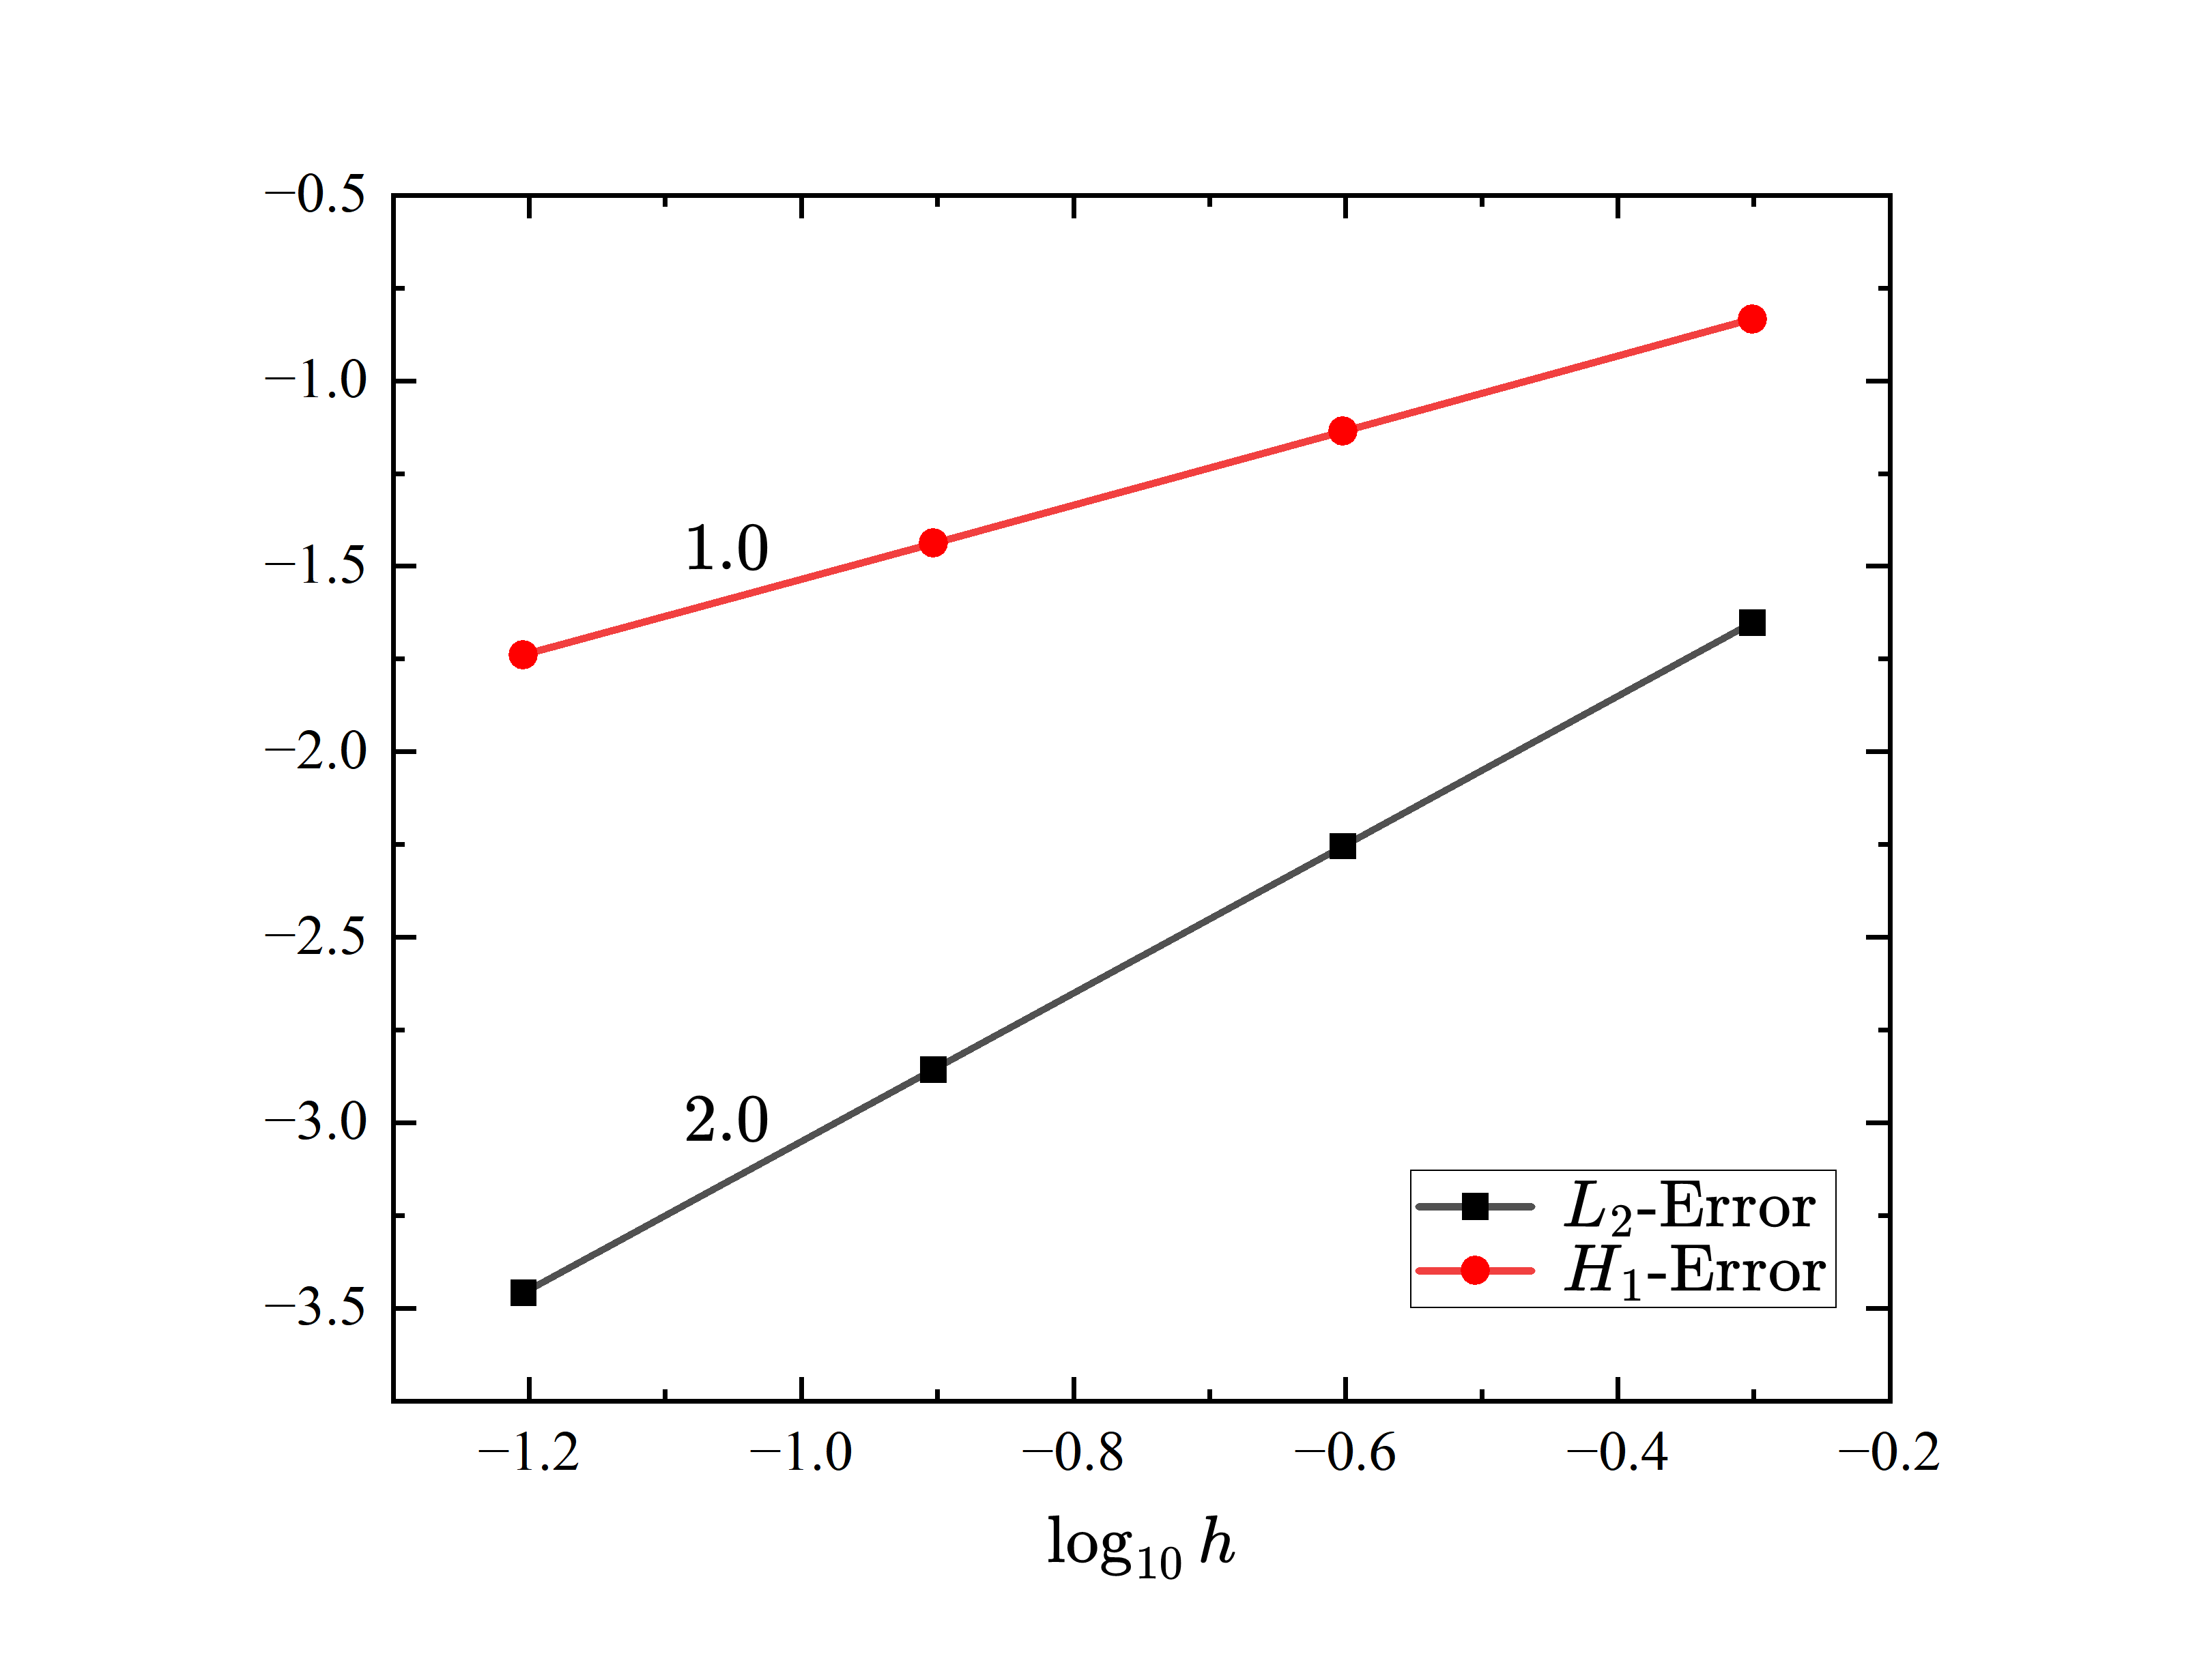
\includegraphics[scale=0.38]{fig/Tri3_连续解_H1L2_均布(8-64_ndiv).png}
\caption{\centering{一维弦自由横向振动问题采用Tri3单元计算的误差收敛结果}}
\label{fg:yiweixiansanjiedianL2}
\end{figure}

当我们采用六节点三角形单元网格进行离散时该问题时，
图\ref{fg:yiweixianliujiedianweiyitu}为该节点离散情况下的位移计算结果，图中所示都具有很好的稳定性。
同时，它的位移误差和能量误差也均能达到理论收敛率，如图\ref{fg:yiweixianliujiedianL2}所示。

\begin{figure}[!h]
    \centering
        \begin{tabular}{c@{\hspace{20pt}}c}
            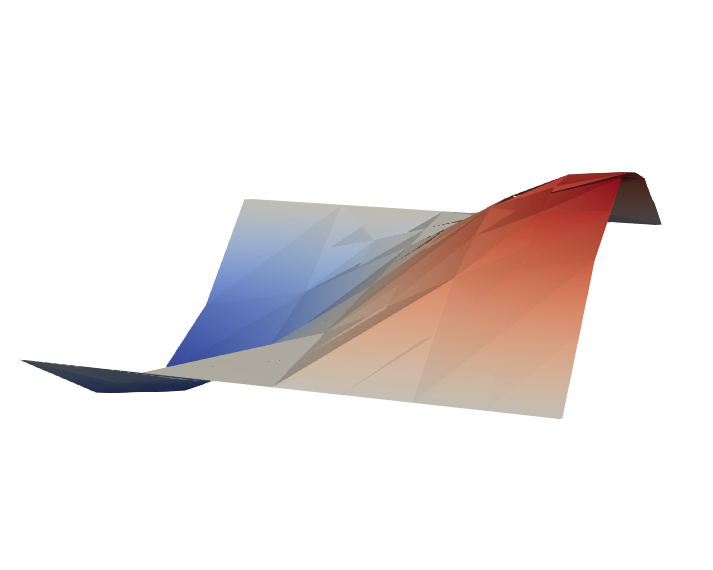
\includegraphics[width=0.4\textwidth]{fig/Tri6_uniform_4.png} &
            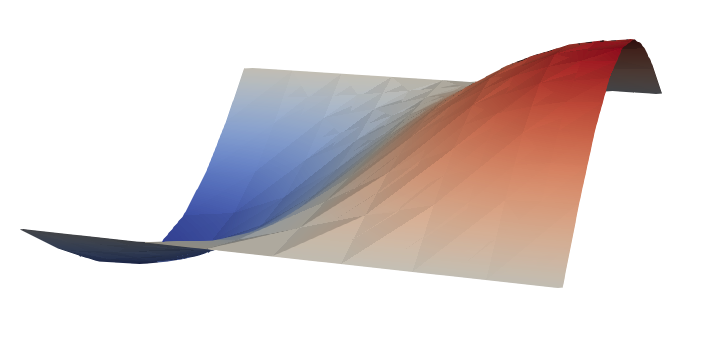
\includegraphics[width=0.4\textwidth]{fig/Tri6_uniform_8.png} \\
            $5\times5$ & $9\times9$ \\
            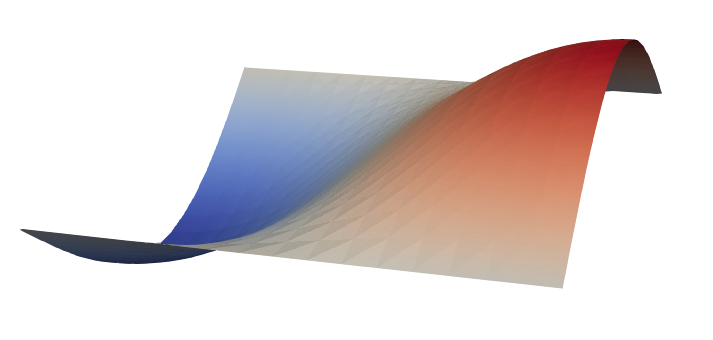
\includegraphics[width=0.4\textwidth]{fig/Tri6_uniform_16.png} &
            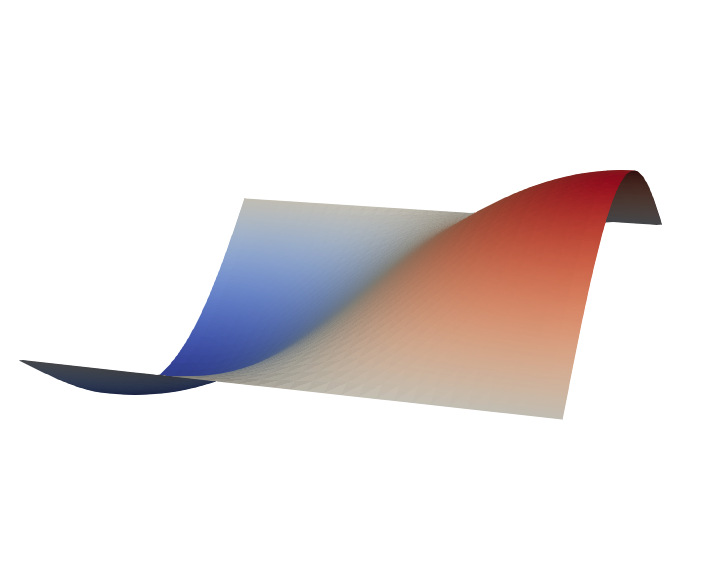
\includegraphics[width=0.4\textwidth]{fig/Tri6_uniform_32.png} \\
            $17\times17$ & $33\times33$ \\
        \end{tabular}
        \caption{一维弦自由横向振动问题六节点单元计算位移图}\label{fg:yiweixianliujiedianweiyitu}
\end{figure}

\begin{figure}[!h]
    \centering
    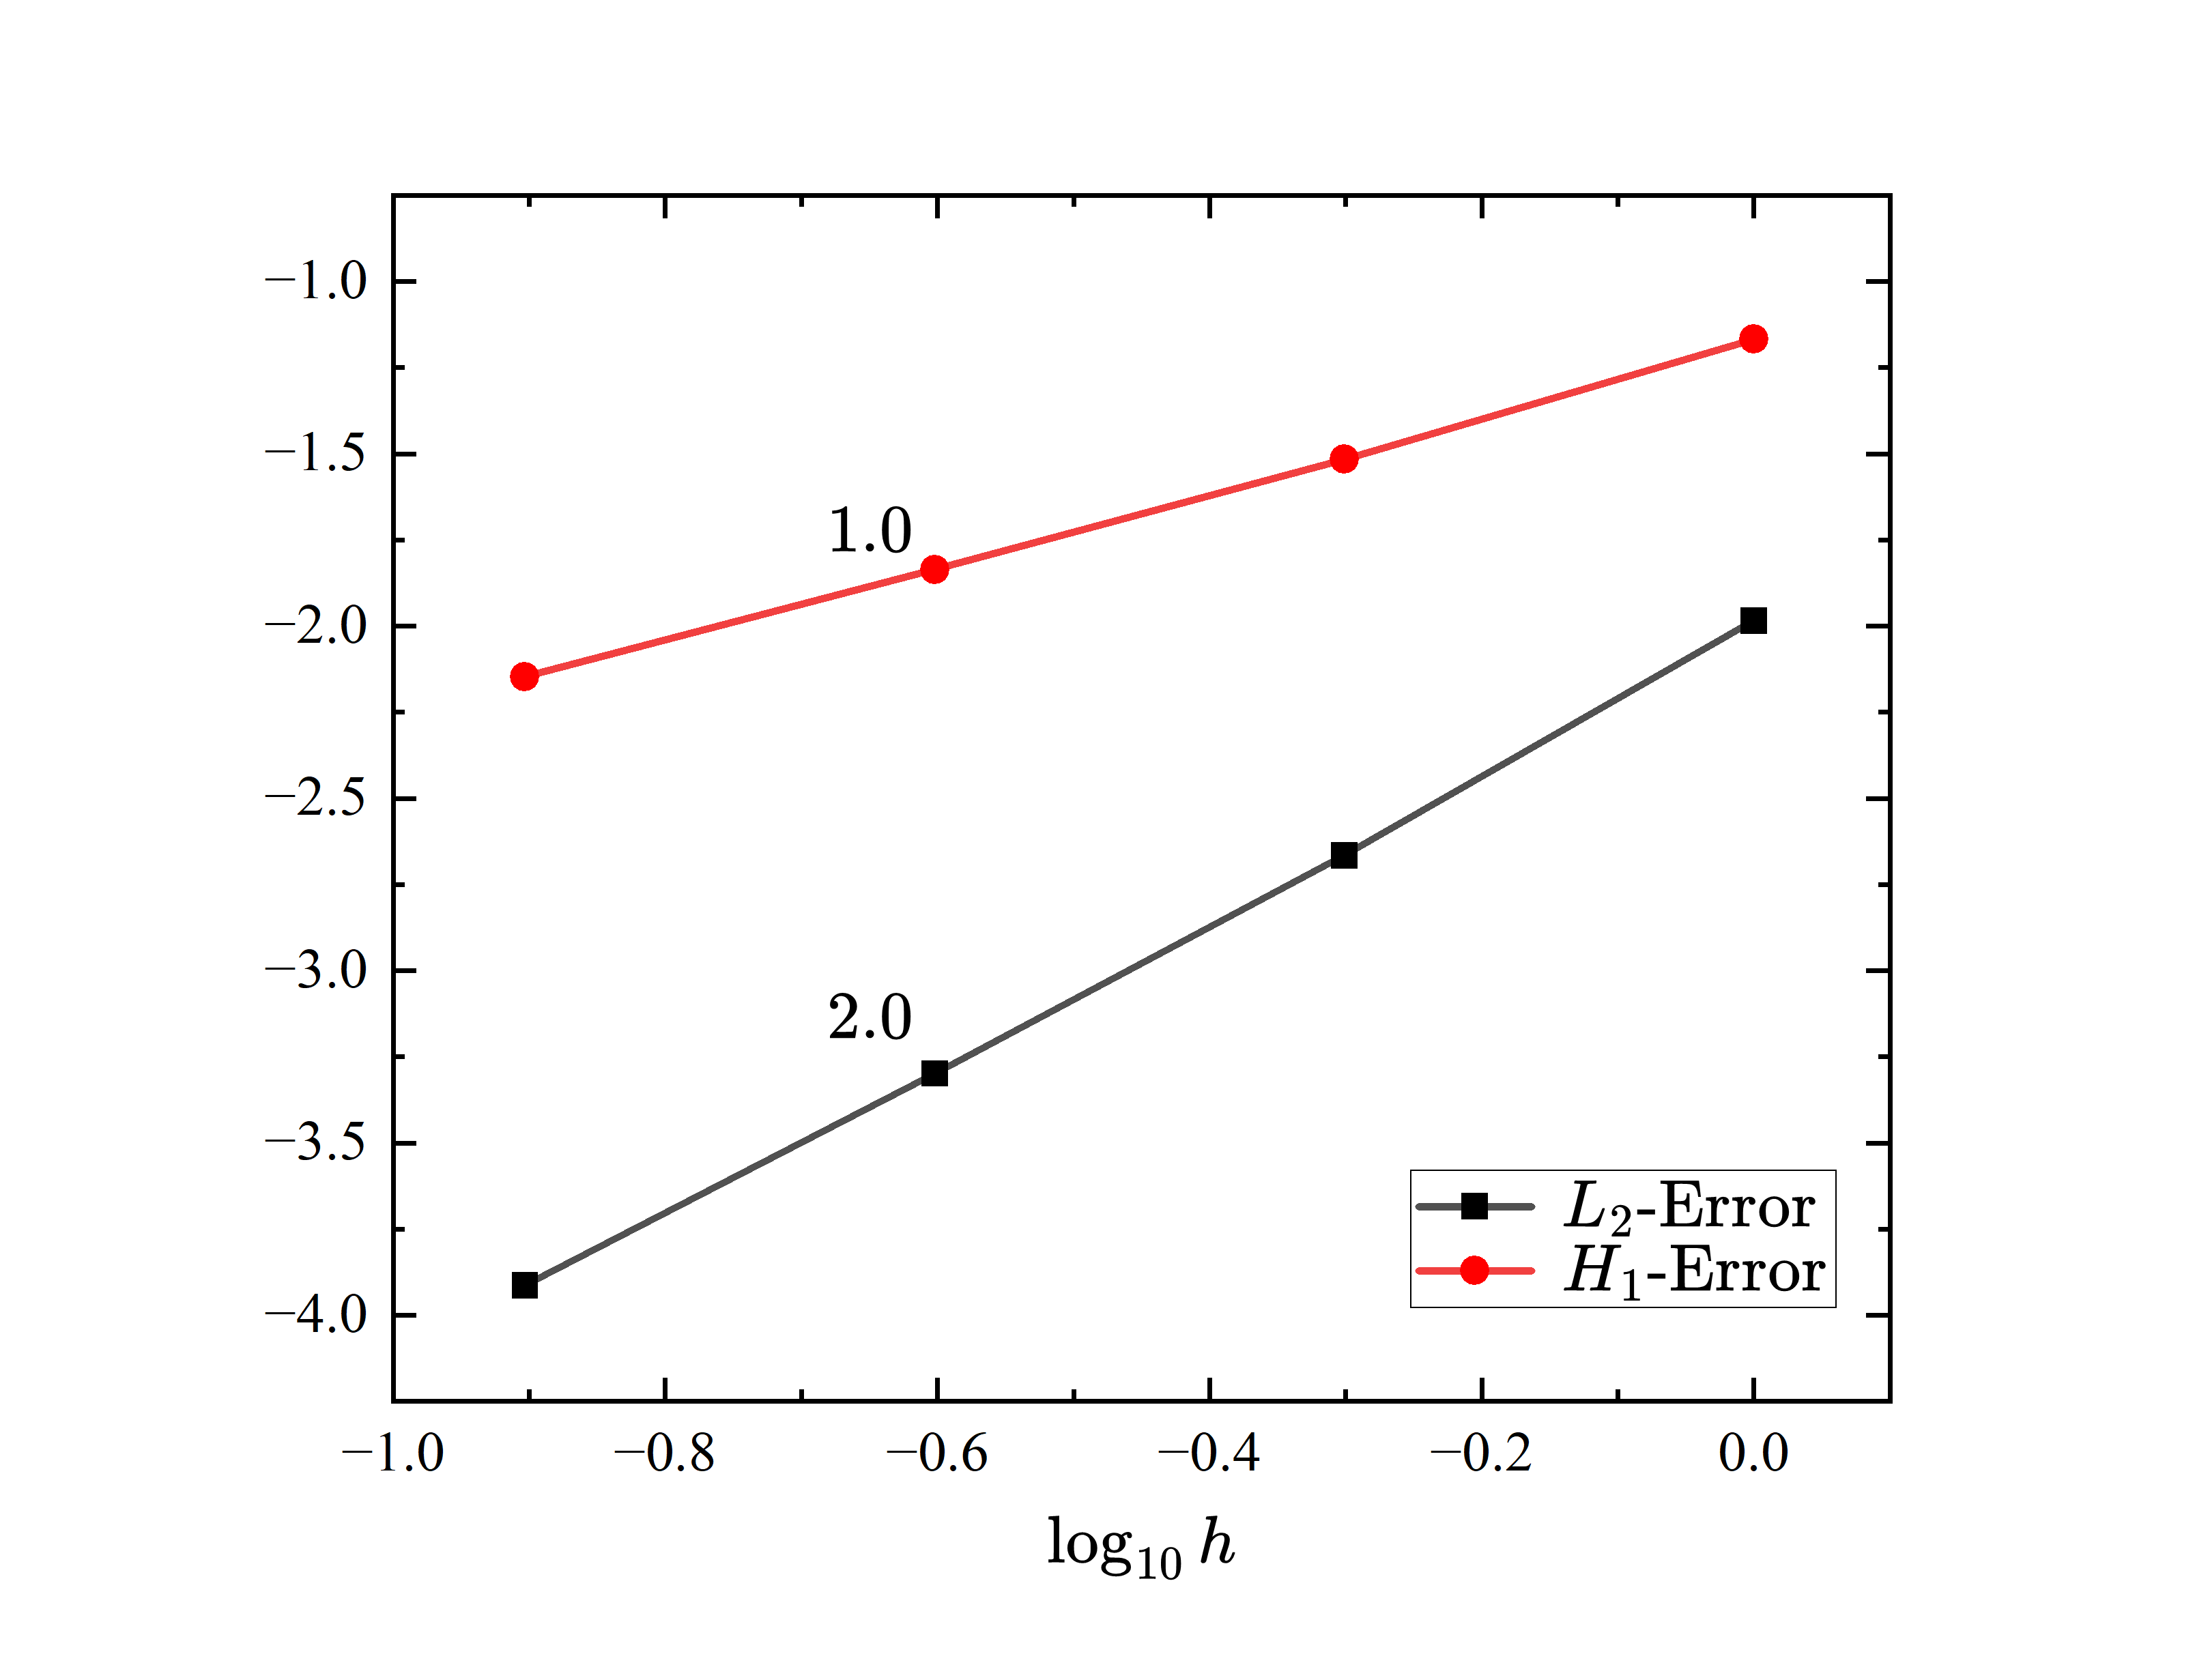
\includegraphics[scale=0.38]{fig/Tri6_连续解_H1L2_均布(4-32_ndiv).png}
\caption{\centering{一维弦自由横向振动问题采用Tri6单元计算的误差收敛结果}}
\label{fg:yiweixianliujiedianL2}
\end{figure}

同样采用Birefine生成不规则的网格来测试一维弦的横向自由振动问题，
根据数值算例的精确解来对该解可能产生误差的部分做refine处理。
生成Birefine的网格图如下：
 
\begin{figure}[!h]
    \centering
        \begin{tabular}{c@{\hspace{20pt}}c}
            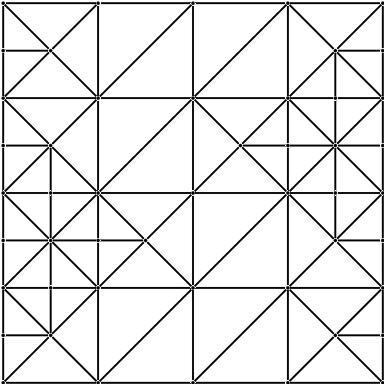
\includegraphics[width=0.3\textwidth]{fig/square_4_r0_refined.png} &
            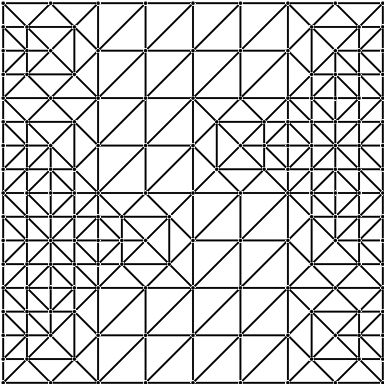
\includegraphics[width=0.3\textwidth]{fig/square_4_r1_refined.png} \\
            BiRefine & 1次Refine \\
            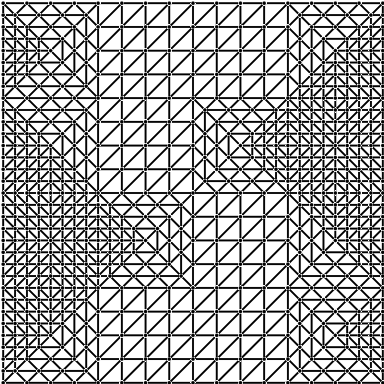
\includegraphics[width=0.3\textwidth]{fig/square_4_r2_refined.png} &
            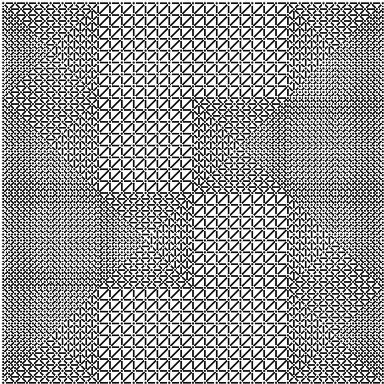
\includegraphics[width=0.3\textwidth]{fig/square_4_r3_refined.png} \\
            2次Refine & 3次Refine \\
        \end{tabular}
        \caption{弹性材料波动问题节点模型}\label{fg:Birefine_Continuous}
\end{figure}

根据上述的BiRefine生成的网格进行离散计算，
图\ref{fg:Birefine_ContinuousL2}为采用上述四个疏密不同的离散节点时的位移误差和能量误差的收敛结果。
从图中可以看出采用基于拉格朗日变分方案的数值分析方法在时空域上求解弹性材料波动问题时，
其位移误差和能量误差均能达到理论收敛率。

\begin{figure}[!h]
    \centering
    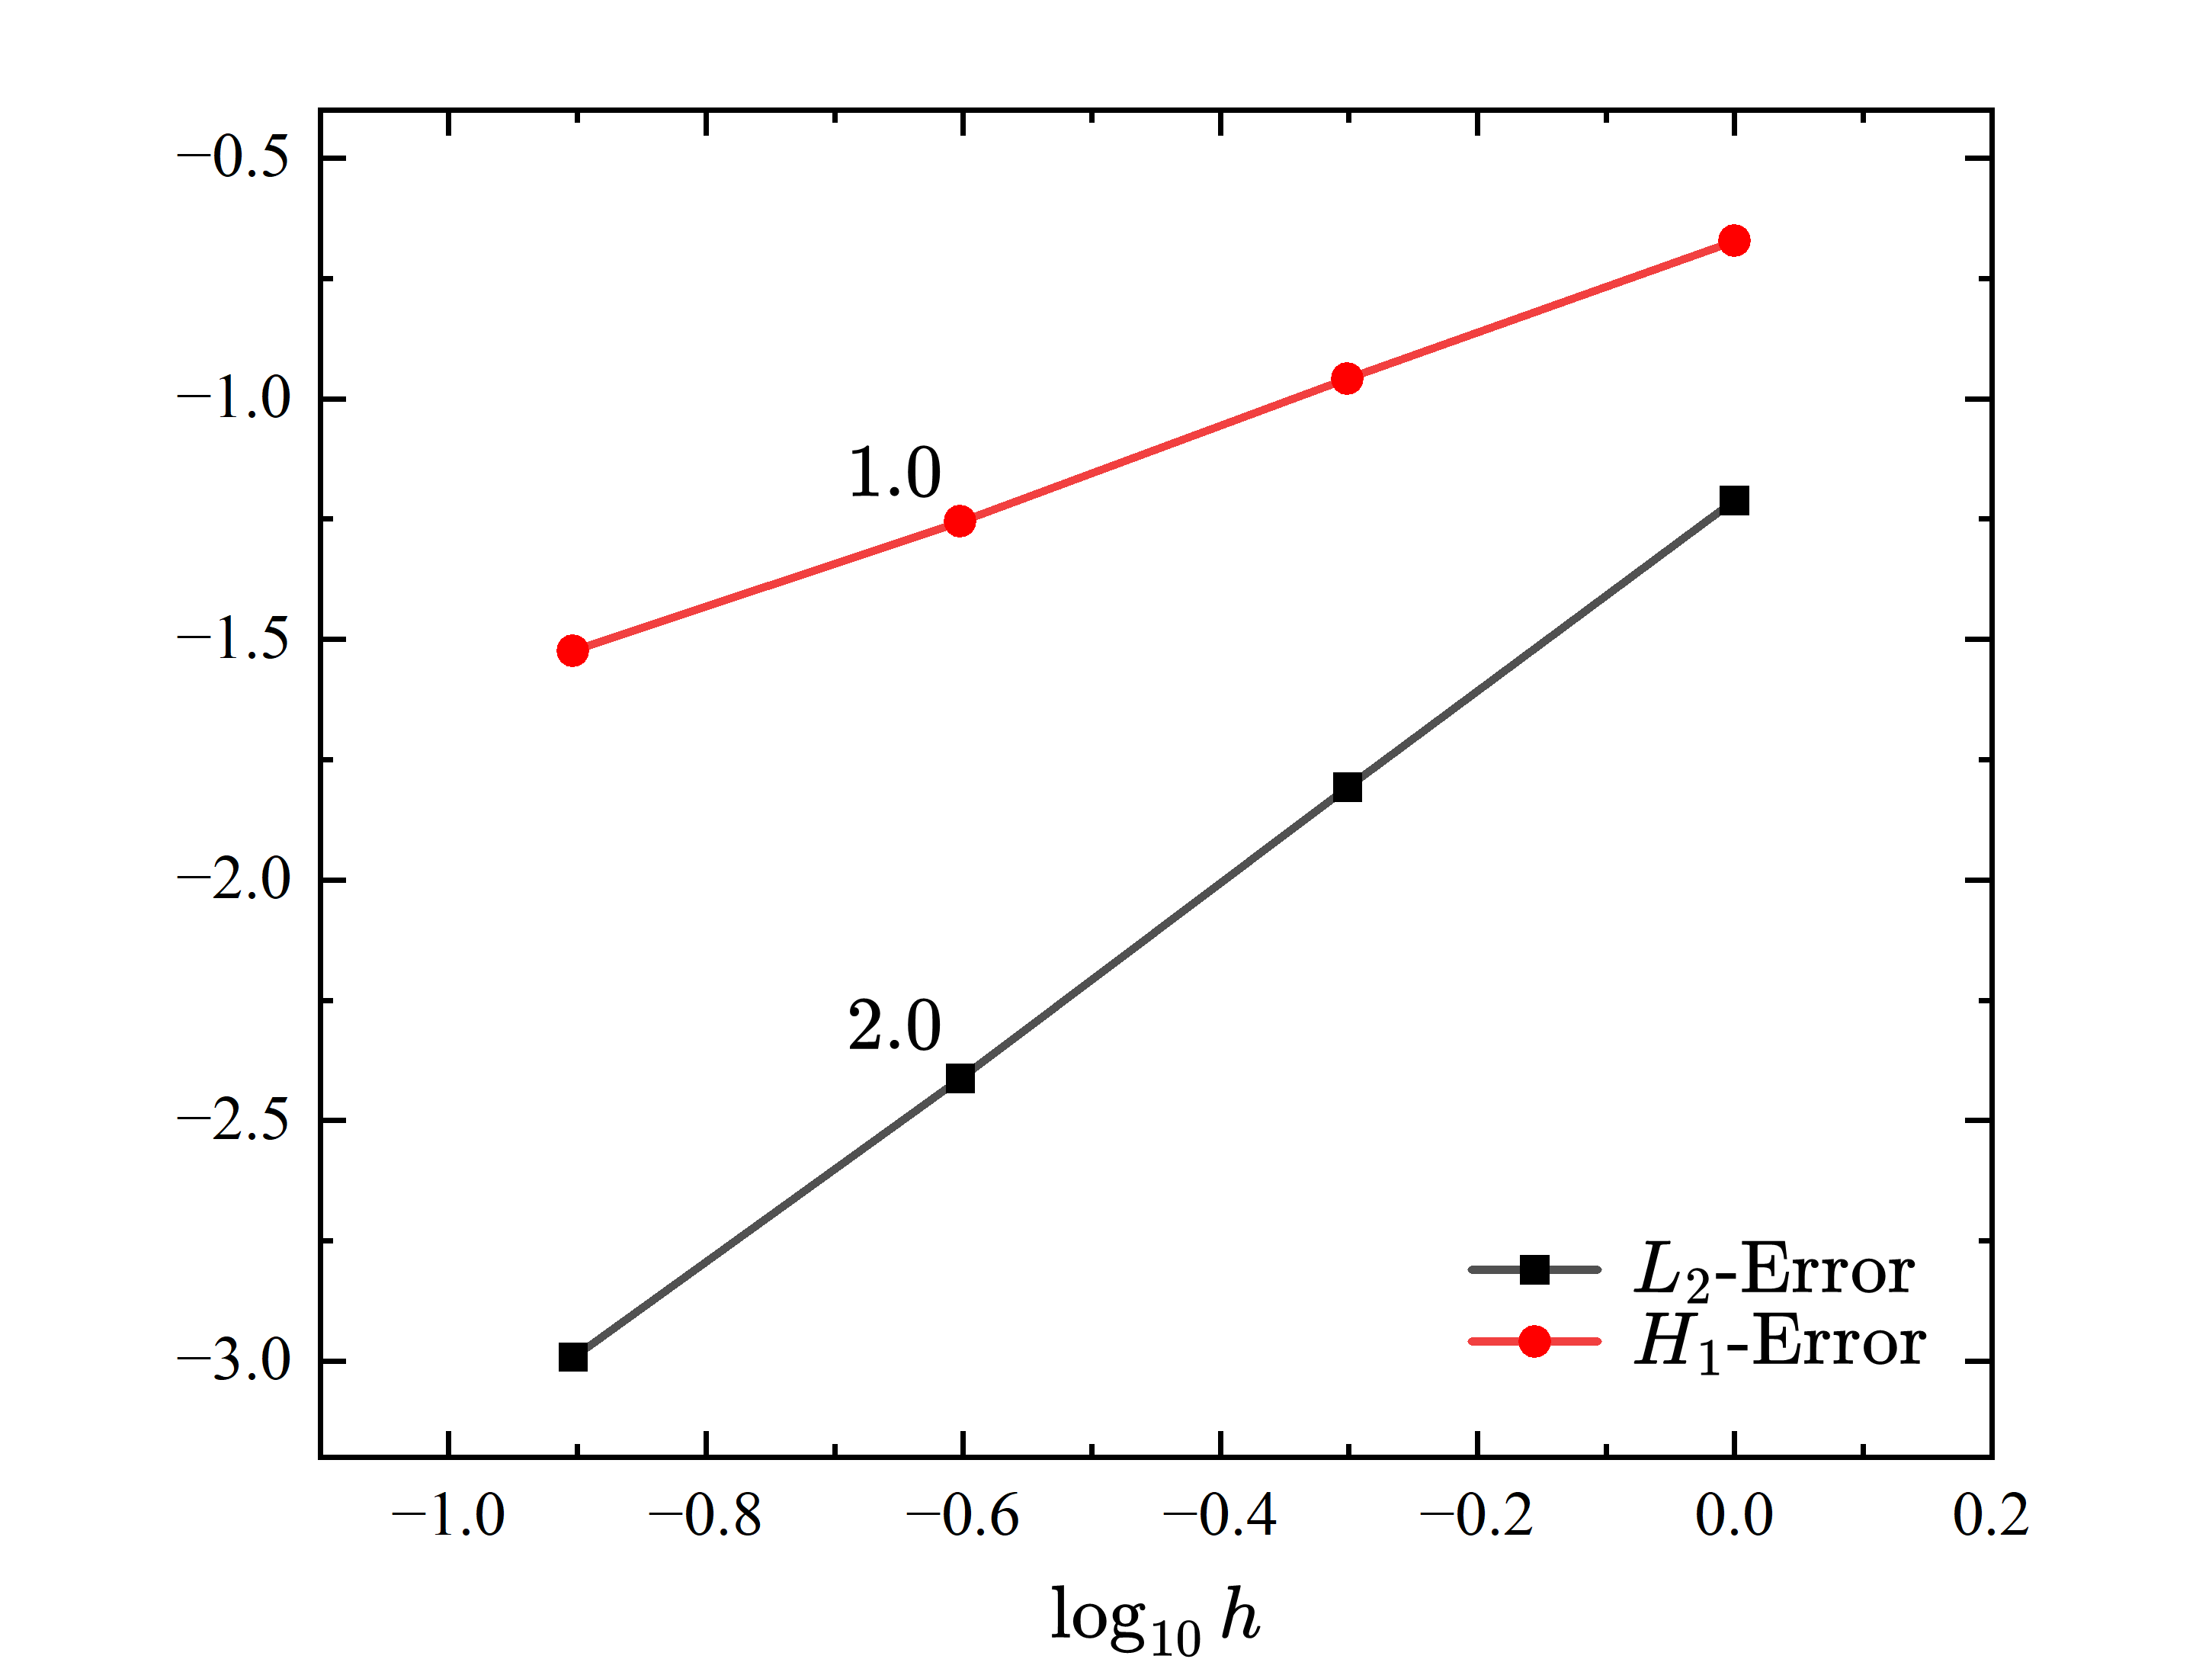
\includegraphics[scale=0.38]{fig/BiRefine_Continuous_4-32.png}
\caption{\centering{一维弦的横向自由振动问题采用BiRefine单元计算的误差收敛结果}}
\label{fg:Birefine_ContinuousL2}
\end{figure}

\clearpage

\section{本章小结}
本章进一步探讨了基于哈密顿原理的拉格朗日变分方案在“1+1”维网格单元的时空混合离散计算。全章主要工作和结论如下：
从一维波动问题的控制方程出发，回顾了结合时间强形式与空间弱形式的经典Newmark迭代法，
分析了其在时间积分域和空间离散域上的耦合特性。
针对完全弱形式伽辽金法在时间末端本质边界条件难以直接施加的痛点，
提出了基于拉格朗日乘子的时空混合变分方案。
通过引入与虚拟变量（类似于动量）等价的拉格朗日乘子，
构造了全新的增广能量泛函。该方案巧妙地将虚位移替换为可数值求解的形式，
从而在对称的时空域中顺利推导并得到了最终统一的有限元离散控制方程，
并且严格给出了该变分框架与经典波动强形式之间的等价性证明。
在数值算例部分，对一维弹性杆撞击刚性墙、弹性材料层波动传导以及一维弦的横向自由振动等经典动力学问题进行了丰富的测试。
结果表明，基于拉格朗日乘子法的变分方案能够实现时空并行分析，
极大提高了计算效率。在位移误差和能量误差的收敛性测试中，
均稳定达到了全阶的最优理论预收敛率。
结合半规则化局部网格自适应加密策略（最长边二分加密），
算法展现了极其优越的局部特征捕捉能力。针对大梯度变化的局域加密能够在保证全局计算效率的同时，
显著抑制非均布网格带来的数值振荡现象，确保了整个动力学推进过程的高精度与数值极强稳定性。

